\documentclass[a4paper,12pt]{article}

\usepackage[T2A]{fontenc}			
\usepackage[utf8]{inputenc}			
\usepackage[english,russian]{babel}	

\usepackage[
bookmarks=true, colorlinks=true, unicode=true,
urlcolor=black,linkcolor=black, anchorcolor=black,
citecolor=black, menucolor=black, filecolor=black,
]{hyperref}

\usepackage{color}
\usepackage{caption}
\DeclareCaptionFont{white}{\color{black}}
\DeclareCaptionFormat{listing}{\colorbox{white}{\parbox{\textwidth}{#1#2#3}}}
\captionsetup[lstlisting]{format=listing,labelfont=white,textfont=white}

\usepackage{amsmath,amsfonts,amssymb,amsthm,mathtools} 
\usepackage{wasysym}

\usepackage{graphicx}
%\usepackage[cache=false]{minted}
\usepackage{cmap}
\usepackage{indentfirst}

\usepackage{listings} 
\usepackage{fancyvrb}

\usepackage{geometry}
\geometry{left=2cm}
\geometry{right=1.5cm}
\geometry{top=1cm}
\geometry{bottom=2cm}

\setlength{\parindent}{5ex}
\setlength{\parskip}{0.5em}

\usepackage{pgfplots}

\begin{document}
	\lstset{ %
		language=C,                 % выбор языка для подсветки (здесь это С)
		basicstyle=\small\sffamily, % размер и начертание шрифта для подсветки кода
		numbers=left,               % где поставить нумерацию строк (слева\справа)
		numberstyle=\tiny,           % размер шрифта для номеров строк
		stepnumber=1,                   % размер шага между двумя номерами строк
		numbersep=5pt,                % как далеко отстоят номера строк от подсвечиваемого кода
		backgroundcolor=\color{white}, % цвет фона подсветки - используем \usepackage{color}
		showspaces=false,            % показывать или нет пробелы специальными отступами
		showstringspaces=false,      % показывать или нет пробелы в строках
		showtabs=false,             % показывать или нет табуляцию в строках
		frame=single,              % рисовать рамку вокруг кода
		tabsize=2,                 % размер табуляции по умолчанию равен 2 пробелам
		captionpos=t,              % позиция заголовка вверху [t] или внизу [b] 
		breaklines=true,           % автоматически переносить строки (да\нет)
		breakatwhitespace=false, % переносить строки только если есть пробел
		escapeinside={\%*}{*)}   % если нужно добавить комментарии в коде
	}
	
	% Титульный лист
	\begin{figure}[h!]
		\begin{center}
			{
\includegraphics[scale = 0.4]{titul.jpg}}
			\label{titul}
		\end{center}
	\end{figure}
	
	\vspace*{15mm} 
	
	\huge
	\begin{center}
		Дисциплина: <<Моделирование>>
	\end{center}
	
	\begin{center}
		Лабораторная работа №5
	\end{center}

	
	\huge
	\begin{center}
		Тема работы:\\
		<<Исследование математической модели на основе технологии вычислительного эксперимента.>>
	\end{center}
	\vspace*{25mm} 
	
	\large
	\begin{flushright}
		Студент: Левушкин И. К. \\
		Группа: ИУ7-62Б \\
		Преподаватель: Градов В. М. \\
	\end{flushright}
	
	\vspace*{25mm}
	\begin{center}
		Москва, 2020 г.  
	\end{center}
	\thispagestyle{empty}
	
	
	\newpage
	
	\section*{Цель работы}
	
	Получение навыков проведения исследований компьютерной математической модели, построенной на квазилинейном уравнении параболического типа.
	Исследование проводится  с помощью программы, созданной в лабораторной работе №4.
	
	\section*{Исходные данные}
	
	\begin{enumerate}
		\item Значения параметров (все размерности согласованы)
		
		$k(T) = a_1 (b_1 + c_1 T^{m_1})$, Вт/см К,
		
		$c(T) = a_2 + b_2 T^{m_2} - \frac{c_2}{T^2}$, Дж/см$^3$К.
		
		Порядки величин (как в лаб. работе №4):
		
		$a_1 = 0.0134, b_1 = 1, c_1 = 4.35 10^{-4}, m_1 = 1,$
		
		$a_2 = 2.049, b_2 = 0.563 10^{-3}, c_2 = 0.528 10^5, m_2 = 1.$
		
		$\alpha (x) = \frac{c}{x - d}$.
		
		Порядки величин (как в лаб. работе №4):
		
		$\alpha_0 = 0.05$ Вт/см$^2$ К,
		
		$\alpha_N = 0.01$ Вт/см$^2$ К,
		
		$l = 10$ см,
		
		$T_0 = 300$ К,
		
		$R = 0.5$ см,
		
		\item Поток тепла $F(t)$ при $x = 0$
		
		$F(t) = \frac{F_{max}}{t_{max}}t e^{-(\frac{t}{t_{max}} - 1)}$, где $F_max, t_max$ - амплитуда импульса потока и время ее достижения (Вт/см$^2$ и с).
		
	\end{enumerate}

	\newpage

	\section*{Результаты работы}
	
	\subsection*{Задание 1.}
	
	
	\textit{Провести исследование по выбору оптимальных шагов по времени $\tau$ и пространству $h$. Шаги должны быть максимально большими при сохранении устойчивости разностной схемы и заданной точности расчета.}
	
	\textit{Рассмотреть влияние на получаемые результаты амплитуды импульса $F_{max}$ и  времени $t_{max}$ (определяют крутизну фронтов и длительность импульса).}
	
	\textit{Точность расчета можно оценить разными способами.
		\begin{enumerate}
			\item Уменьшая шаги и наблюдая сходимость решений, как это делалось в лаб. работе №1.
			\item Проверяя, соблюдается ли при выбранных $h, \tau$ баланс мощности после выхода на стационарное распределение температуры (в установившемся режиме), реализующееся при $F(t) = const$, т.е. в этом режиме  должно выполняться условие: подводимая мощность  равна отводимой. Имеем
		\end{enumerate}
	}

	\[\pi R^2 (F_0 - F_N) = 2\pi R \int_{0}^{l}\int \alpha \left[T(x, t_m) - T_0\right]dx,\]
	
	\textit{окончательно}
	
	\begin{equation}\label{ris:f}
		\frac{F_0 - F_N}{\frac{2}{R} \int_{0}^{l}\int \alpha \left[T(x, t_m) - T_0\right]dx} - 1 \leqslant \varepsilon.
	\end{equation}

	\textit{Задать точность $\varepsilon$ примерно $10^-2$. Здесь $t_m$  - время выхода на стационарный режим, т.е. когда температура перестает меняться с за-данной точностью (см. лаб. работу №4).}
	
	\textit{Замечание. Варьируя параметры задачи, следует иметь ввиду, что решения, в ко-торых температура превышает значения примерно 2000К, физического смысла не имеют и практического интереса не представляют.}
	
	\subsubsection*{Решение}
	
	Начнем исследование по выбору оптимальных шагов по времени и пространству, проверяя выполнение неравенства (\ref{ris:f}) из 2 способа на следующем диапазоне шагов: по $t$: $\tau = 1, 2, ..., 10$ сек, по $x$: $h = 0.1, 0.2, ..., 1$ см. $F(t) = const = F_0$.
	
	Ниже представлены результаты выполнения/не выполнения неравенства (\ref{ris:f}) на заданном диапазоне шагов в виде множества точек на графике $\tau(h)$, где точки $(h_i, \tau_i)$ означают, что при шагах $h = h_i, \tau = \tau_i$ неравенство выполняется.
	
	\begin{figure}[h!]
		\begin{center}
			{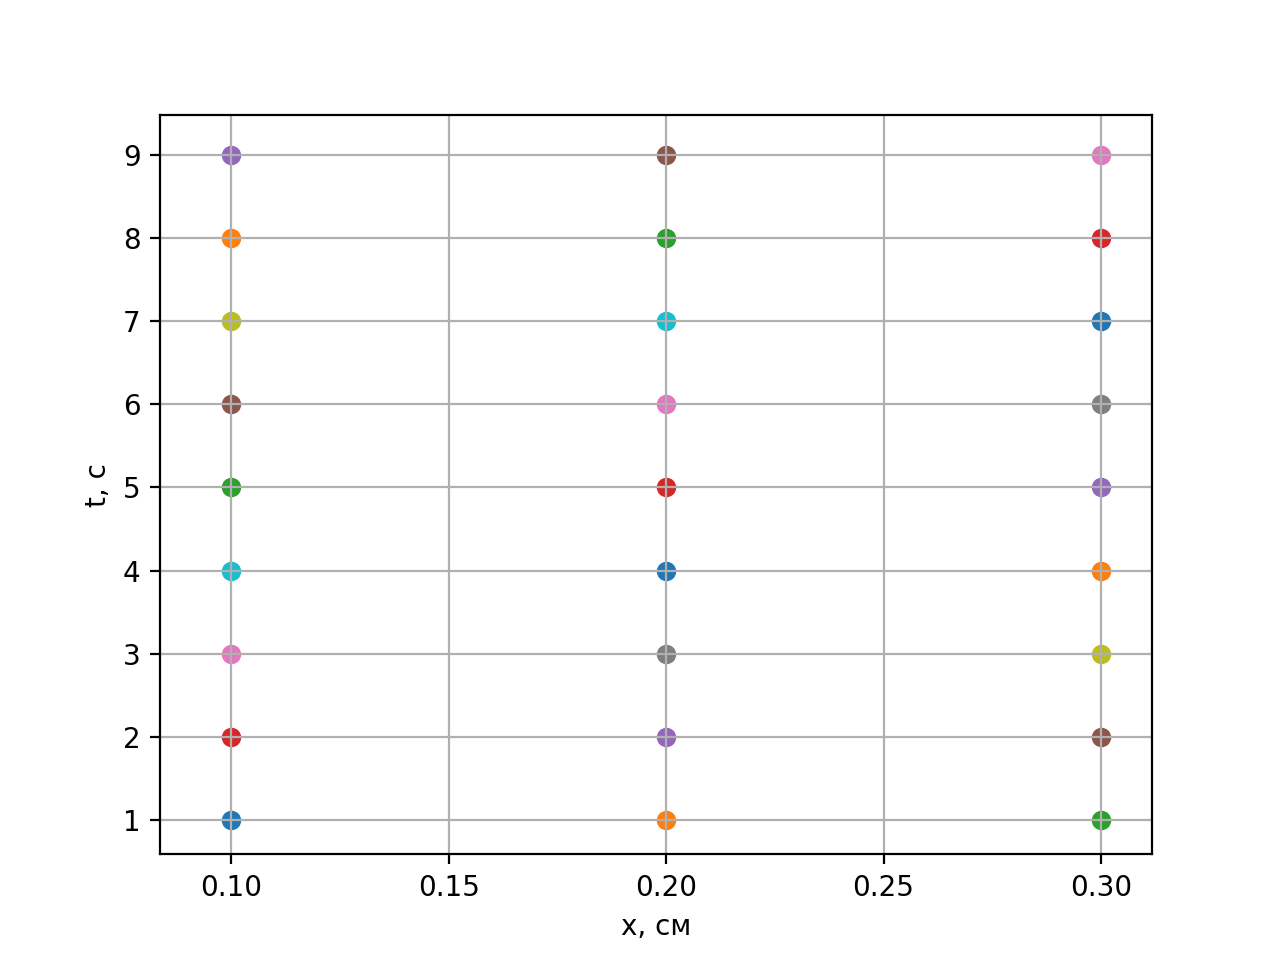
\includegraphics[scale = 0.6]{1.png}}
			\label{ris:1}
		\end{center}
		\caption{Выполнение неравенства (\ref{ris:f}) при определенных шагах}
	\end{figure}
	
	Отсюда видно, что при $h > 0.3$ см, баланс мощности после выхода на стационарное распределение температуры не соблюдается. Также, из данного эксперимента вытекает, что баланс мощности после выхода на стационарное распределение температуры не зависит от шага по времени. Это обусловлено тем, что параметры неравенства (\ref{ris:f}) не зависят от $\tau$.
	
	Таким образом, остановимся на $h = 0.3$ см и начнем уменьшать шаги по времени.
	
	Для функции $F(t) = \frac{F_{max}}{t_{max}}t e^{-(\frac{t}{t_{max}} - 1)}$, подберем $F_{max} = 30$ Вт/см$^2$, $t_{max} = 20$ с..
	
	Поскольку график функции $F(t) = \frac{30}{20}t e^{-(\frac{t}{20} - 1)} \approx 0$ при $t > 160$ с. (рис. \ref{ris:F(t)}), то будем проводить измерения при $t_i = 18, 72, 144$ с. (поскольку при $t > 160$ стержень уже практически весь остынет и будет нечего сравнивать).
	
	\newpage
	
	\begin{figure}[h!]
		\begin{center}
			{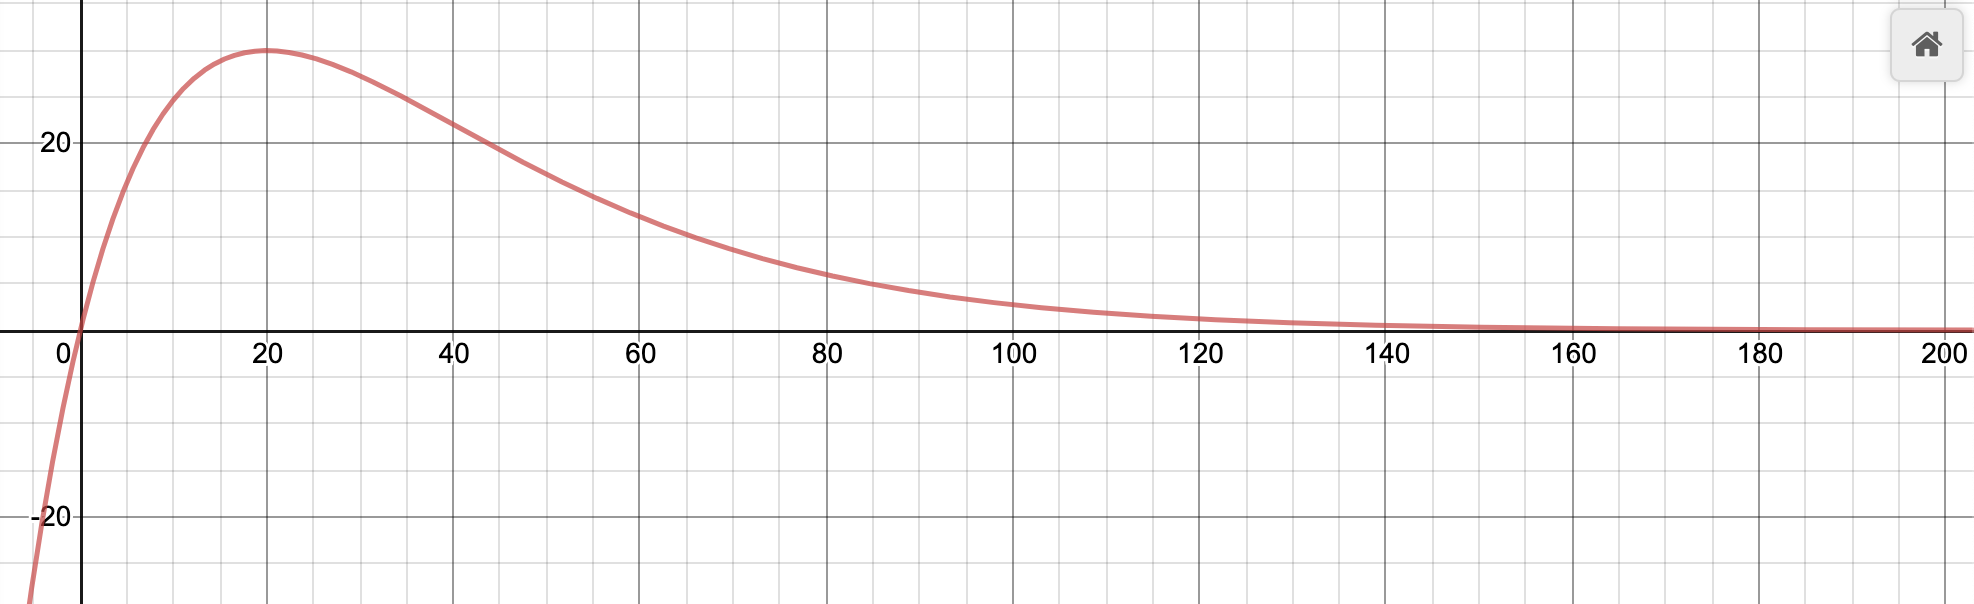
\includegraphics[scale = 0.5]{F(t).png}}
		\end{center}
		\caption{График функции $F(t) = \frac{30}{20}t e^{-(\frac{t}{20} - 1)}$}
		\label{ris:F(t)}
	\end{figure}

	Ниже приведены 3 таблицы для $t_i = 18, 72, 144$ с. соответственно.
	
	Каждая колонка (кроме 1-ой) соответствует значениям функции $T(x, t_i)$ при шагах $\tau_k$ по $t$ и $h = 0.3$ см по $x$.
	
	\begin{figure}[h!]
		\begin{center}
			{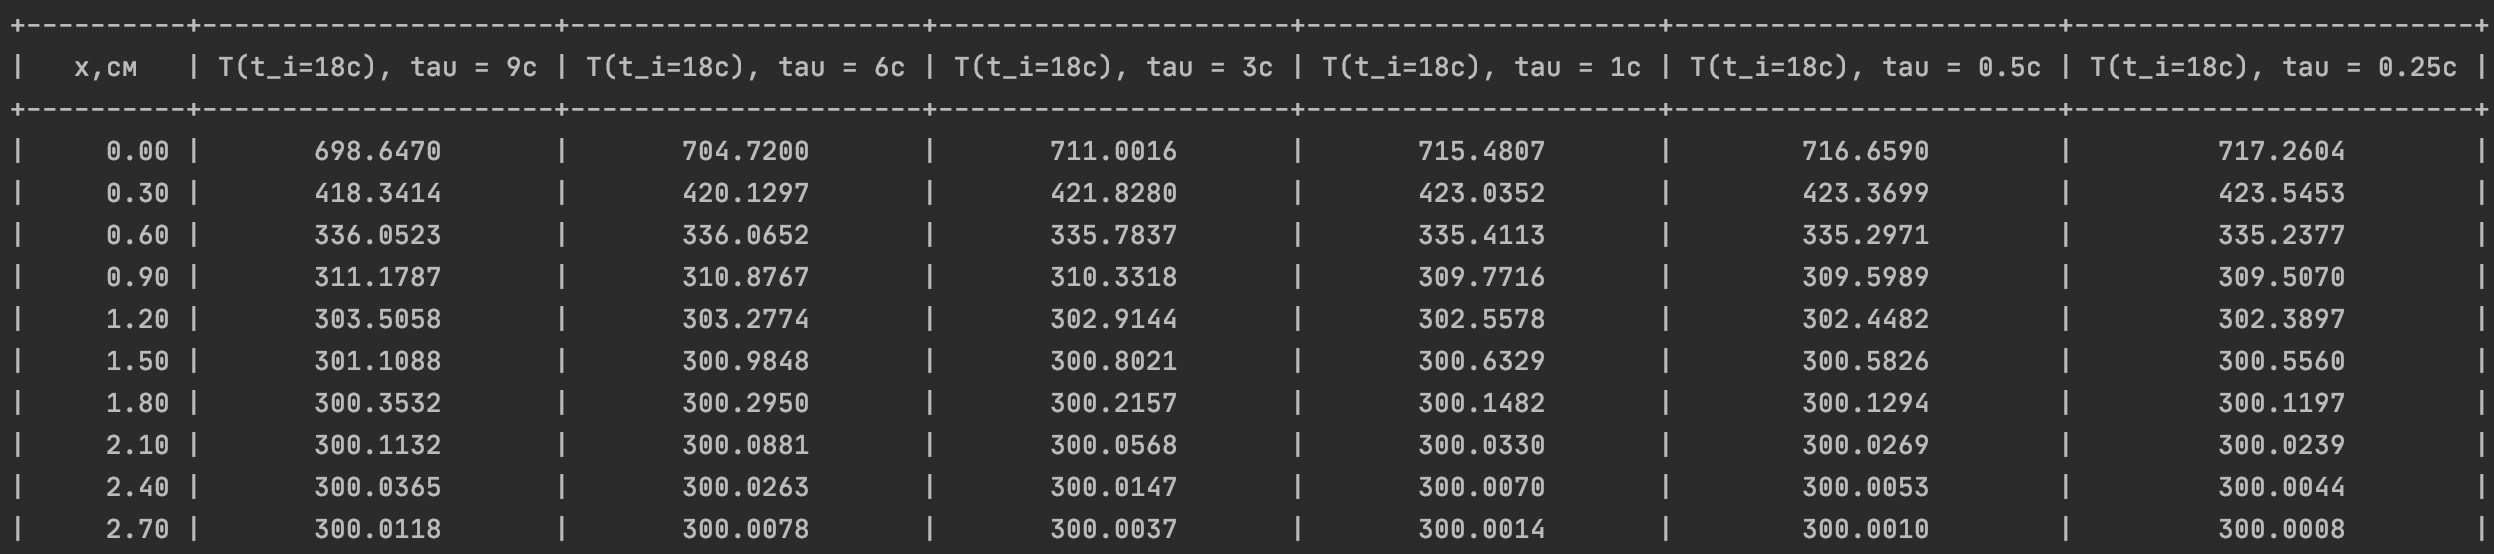
\includegraphics[scale = 0.43]{18.png}}
			\label{table:18}
		\end{center}
		\caption{Таблица $T(x, 18)$. $h = 0.3$ см.}
	\end{figure}

	\begin{figure}[h!]
		\begin{center}
			{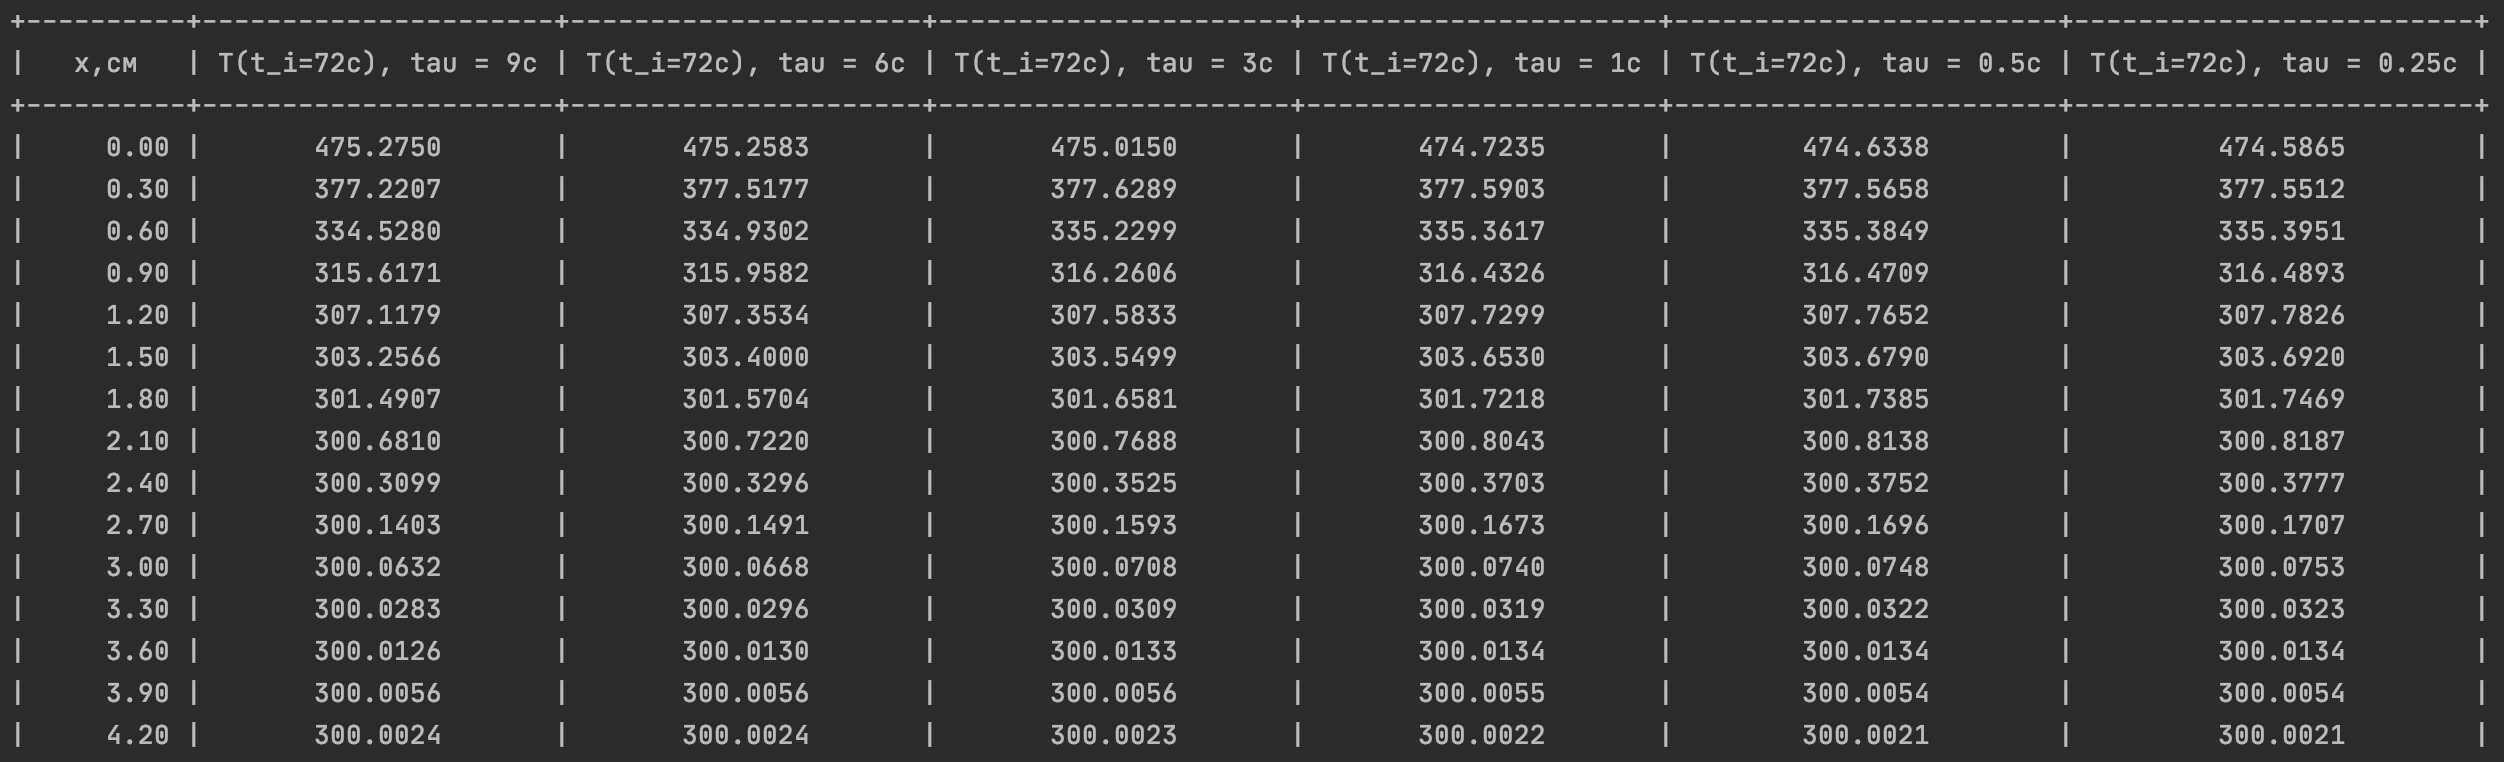
\includegraphics[scale = 0.43]{72.png}}
			\label{table:72}
		\end{center}
		\caption{Таблица $T(x, 72)$. $h = 0.3$ см.}
	\end{figure}

	\newpage

	\begin{figure}[h!]
		\begin{center}
			{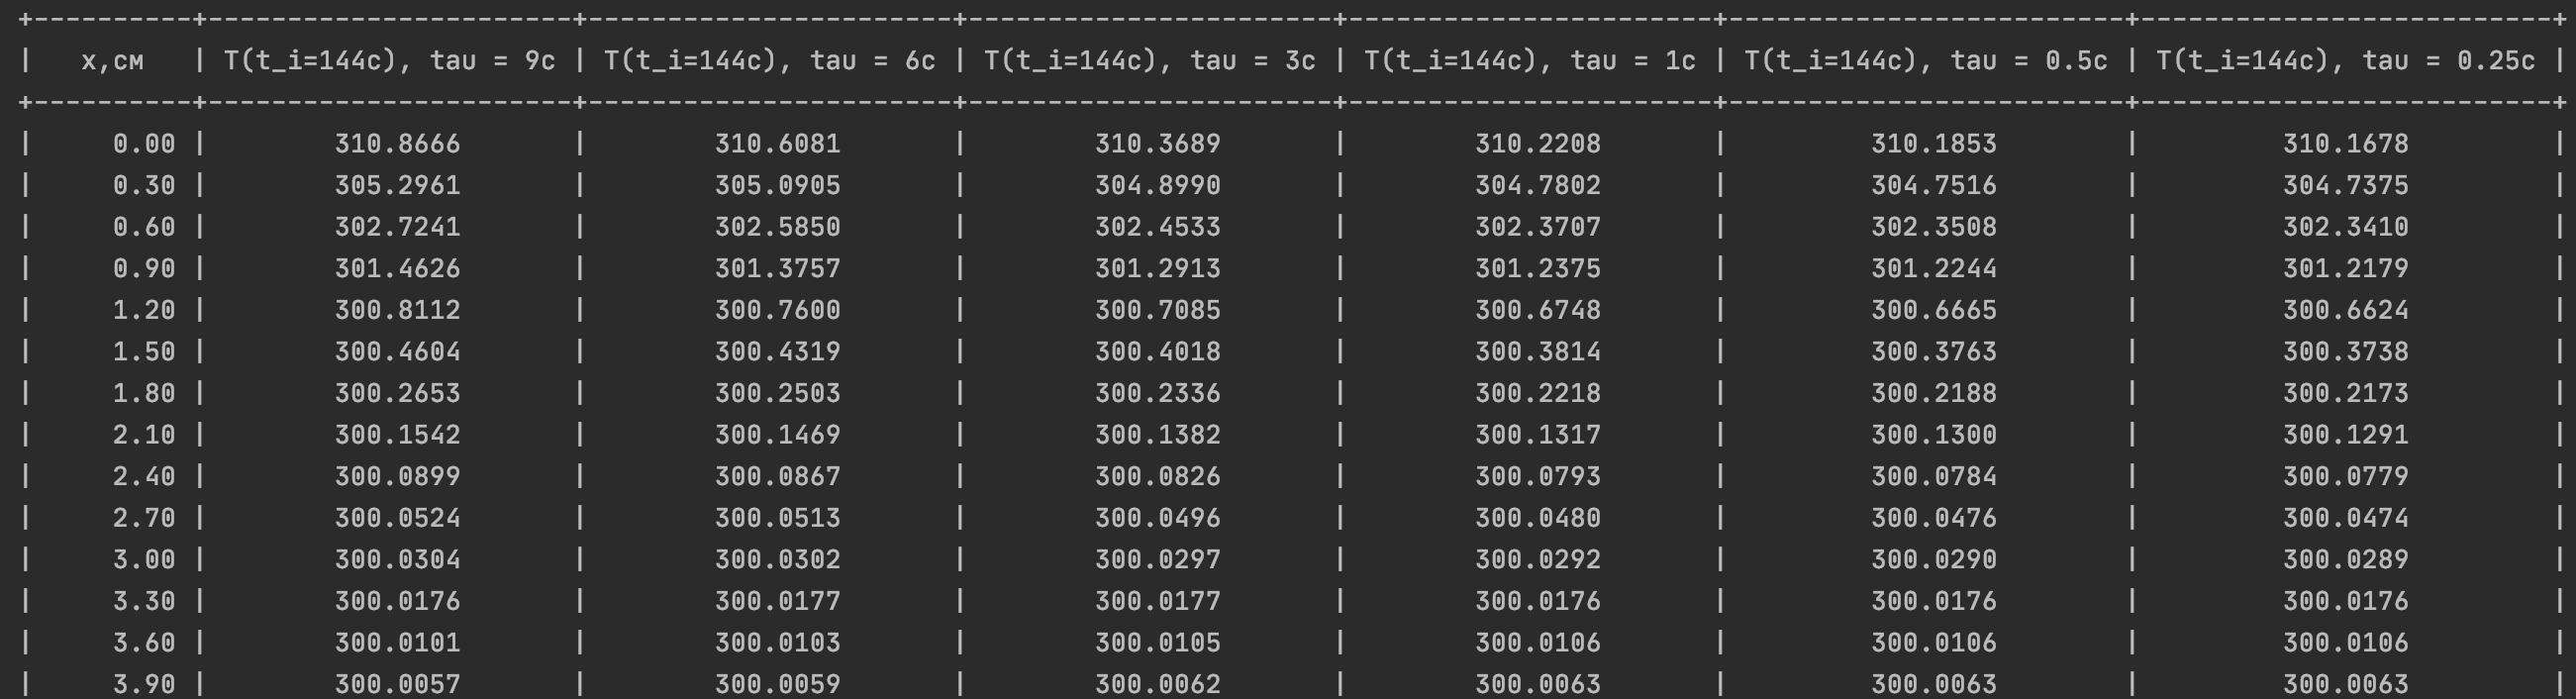
\includegraphics[scale = 0.4]{144.png}}
			\label{table:144}
		\end{center}
		\caption{Таблица $T(x, 144)$. $h = 0.3$ см.}
	\end{figure}

	Фиксируя $x_j$ и сравнивая на этой строке значения $T(x_j, t_i)$ при разных шагах $\tau$ в каждой таблице, придем к выводу, что наиболее оптимальный шаг по времени $\tau = 1$ с., поскольку при $\tau > 1$ значения $T$ далеки от точного, а при $\tau < 1$ различия уже незначительные (наблюдается сходимость решений).
	
	\textit{Пример:}
	
	Фиксируем $x_j = 0.3$ см; 
	
	$T(t_i = 18) = 418.3414, 420.1297, 421.8280, 423.0352, 423.3699, 423.5453$ К 
	
	при  $\tau = 9, 6, 3, 1, 0.5, 0.25$ с. соответственно.
	
	\vspace*{20mm} 
	
	Далее, начнем уменьшать шаги по пространству $h$ при $\tau = 1$ с..
	
	Ниже приведены 3 таблицы для $t_i = 18, 72, 144$ с. соответственно.
	
	Каждая колонка (кроме 1-ой) соответствует значениям функции $T(x, t_i)$ при шагах $h_k$ см по $x$ и $\tau = 1$ с. по $t$.
	
	\begin{figure}[h!]
		\begin{center}
			{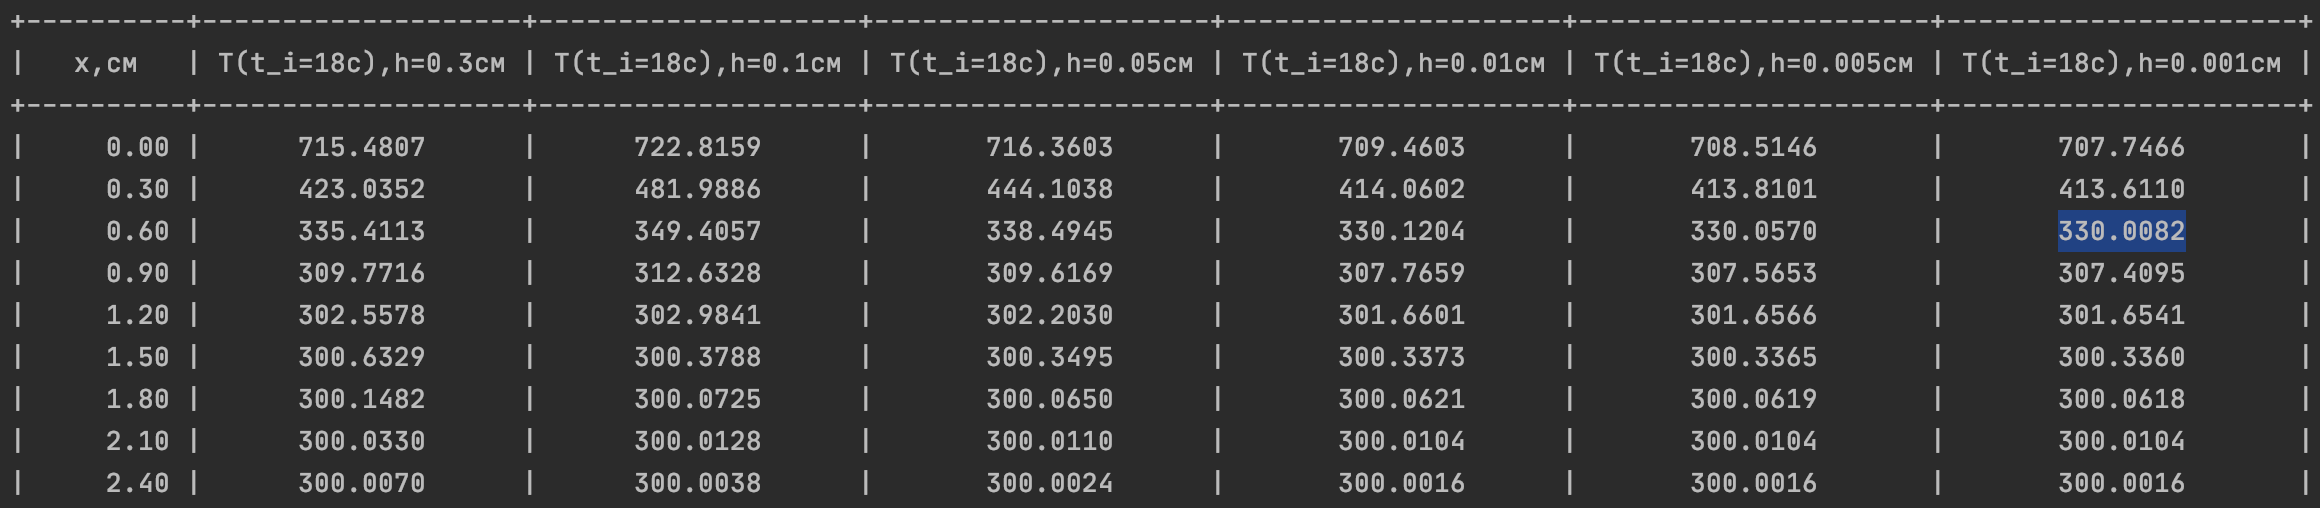
\includegraphics[scale = 0.45]{18_2.png}}
			\label{table:18_2}
		\end{center}
		\caption{Таблица $T(x, 18)$. $\tau = 1$ с.}
	\end{figure}

	\newpage
	
	\begin{figure}[h!]
		\begin{center}
			{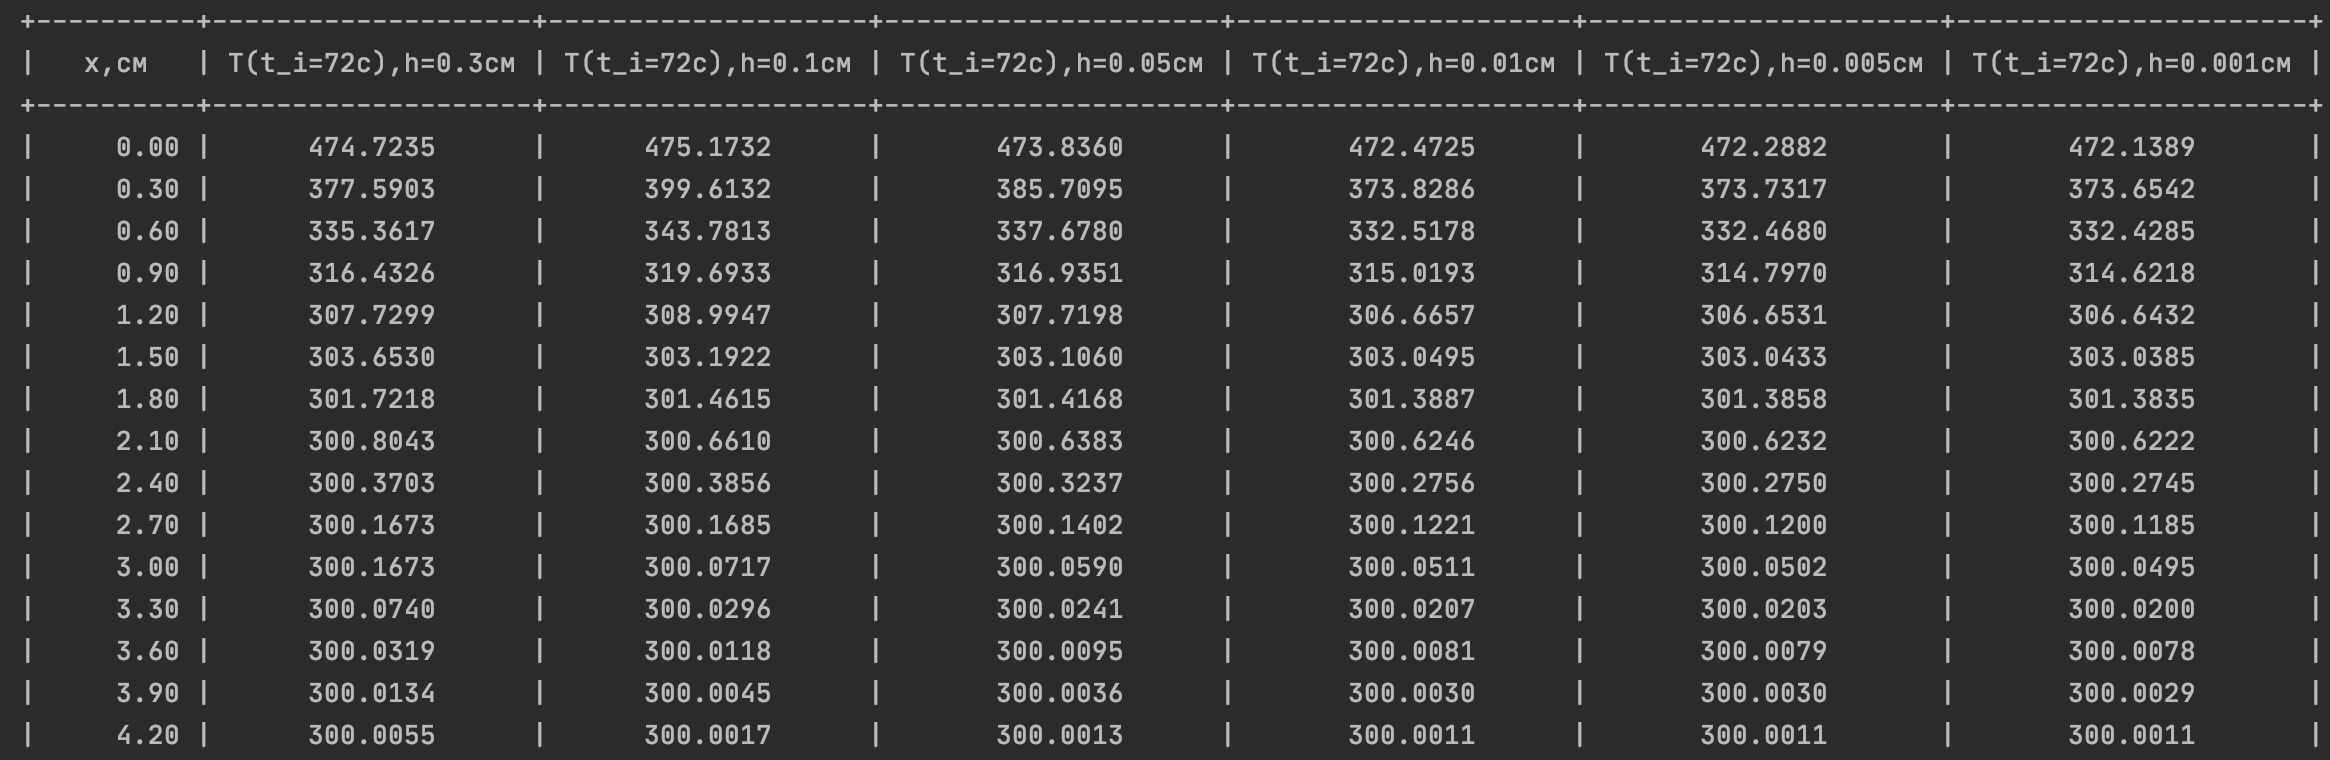
\includegraphics[scale = 0.45]{72_2.png}}
			\label{table:72_2}
		\end{center}
		\caption{Таблица $T(x, 72)$. $\tau = 1$ с.}
	\end{figure}
	
	\begin{figure}[h!]
		\begin{center}
			{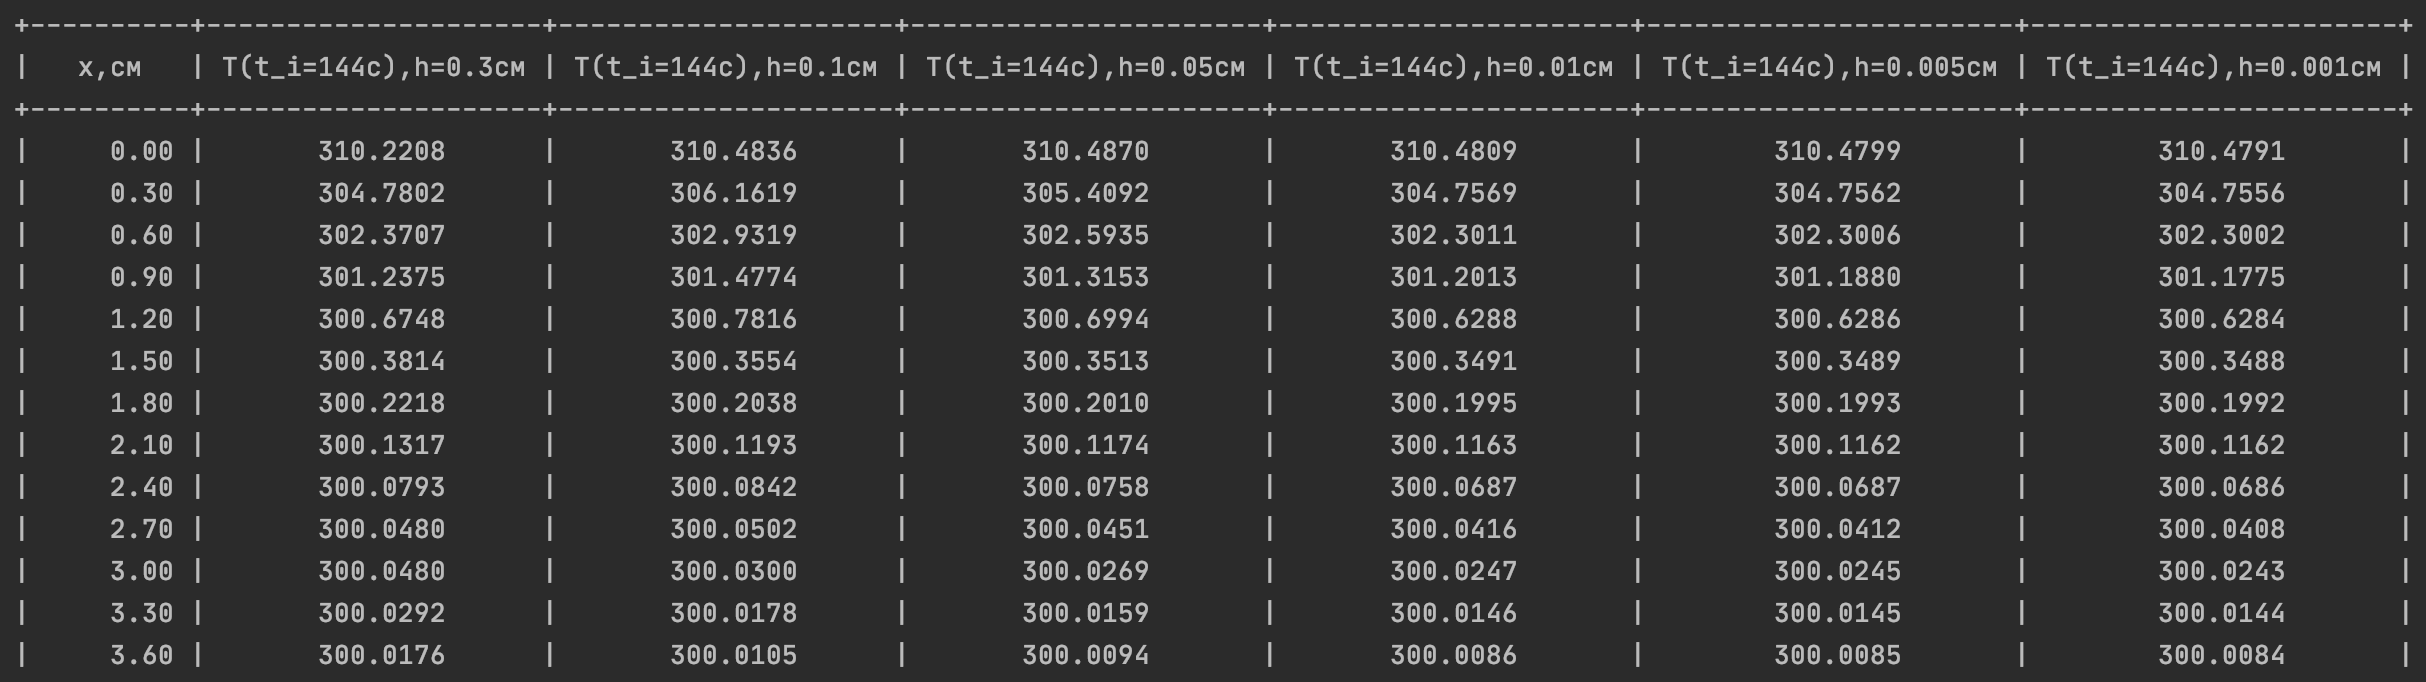
\includegraphics[scale = 0.45]{144_2.png}}
			\label{table:144_2}
		\end{center}
		\caption{Таблица $T(x, 144)$. $\tau = 1$ с.}
	\end{figure}
	
	Фиксируя $x_j$ и сравнивая на этой строке значения $T(x_j, t_i)$ при разных шагах $h$ в каждой таблице, придем к выводу, что наиболее оптимальный шаг по пространству $h = 0.01$ см, поскольку при $h > 1$ значения $T$ далеки от точного, а при $h < 1$ различия уже незначительные (наблюдается сходимость решений).
	
	\textit{Пример: }
	
	Фиксируем $x_j = 0.6$ см; 
	
	$T(t_i = 18) = 335.4113, 349.4057, 338.4945, 330.1204, 330.0570, 330.0082$ К 
	
	при $h = 0.3, 0.1, 0.05, 0.01, 0.005, 0.001$ см., соответственно.
	
	Таким образом, оптимальные шаги:
	
	$\tau = 1.0$ с.
	
	$h = 0.01$ см.
	
	\newpage
	
	При этом $F_{max}$ и $t_{max}$ будут влиять на полученные результаты только в том случае, если сделать их слишком маленькими (близкими к 0). При уменьшении $t_{max}$ будет меняться выбор, какие $t_i$ нужно будет фиксировать для $T(x_j, t_i)$. Поскольку, если задать $t_{max}$ очень маленьким (близким к 0), то стержень быстро остынет и сравнивать будет уже нечего на больших $t_i$.
	
	\textit{Пример:}
	
	Зададим $t_{max} = 0.7$ с.. Тогда график функции $F(t)$ выглядит следующим образом:
	
	\begin{figure}[h!]
		\begin{center}
			{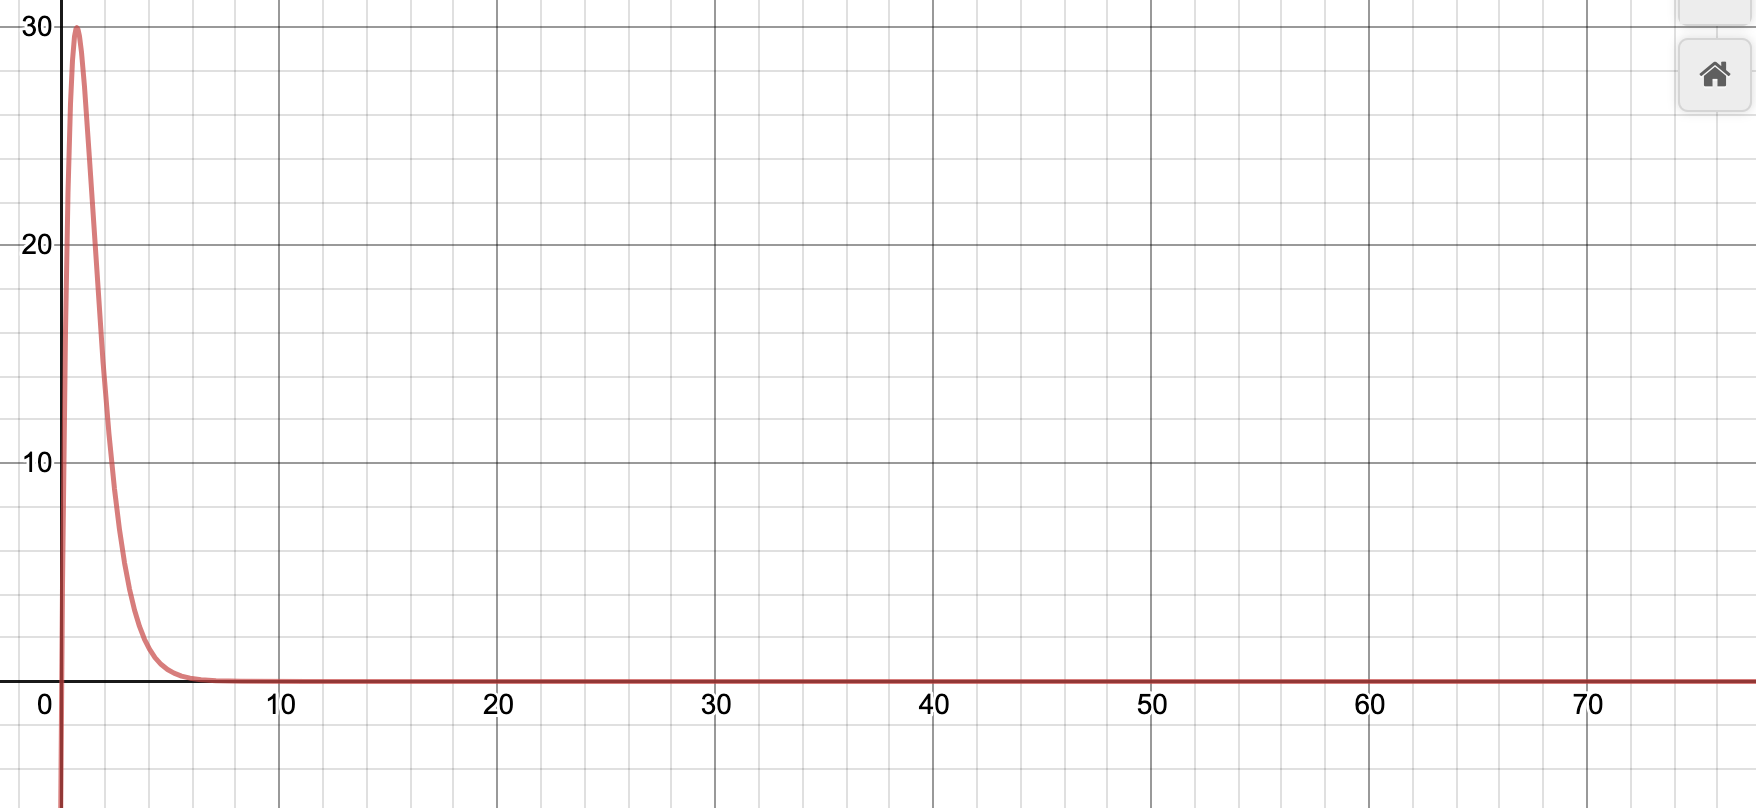
\includegraphics[scale = 0.6]{F(t)_2.png}}
			\label{ris:F(t)_2}
		\end{center}
		\caption{График функции $F(t) = \frac{30}{0.7}t e^{-(\frac{t}{20} - 1)}$}
	\end{figure}

	Где видно, что уже при $t = 9$ с. $F(t) \approx 0$. А значит уже при $t > 20$ (когда стержень практически полностью остынет) температура по всей длине стержня будет практически равна 300 К. Поэтому придется сравнивать только при малых $t_i$. Соответственно, если уменьшить $t_max$ на столько, что оно будет меньше тестируемого шага $\tau$, то и сравнить ничего не получится.
	
	\newpage
	
	То же самое касается и $F_{max}$. Если задать его значение близким к 0, то стержень в принципе не будет нагреваться и сравнивать будет нечего (рис. \ref{ris:F(t)_3}).
	
	\begin{figure}[h!]
		\begin{center}
			{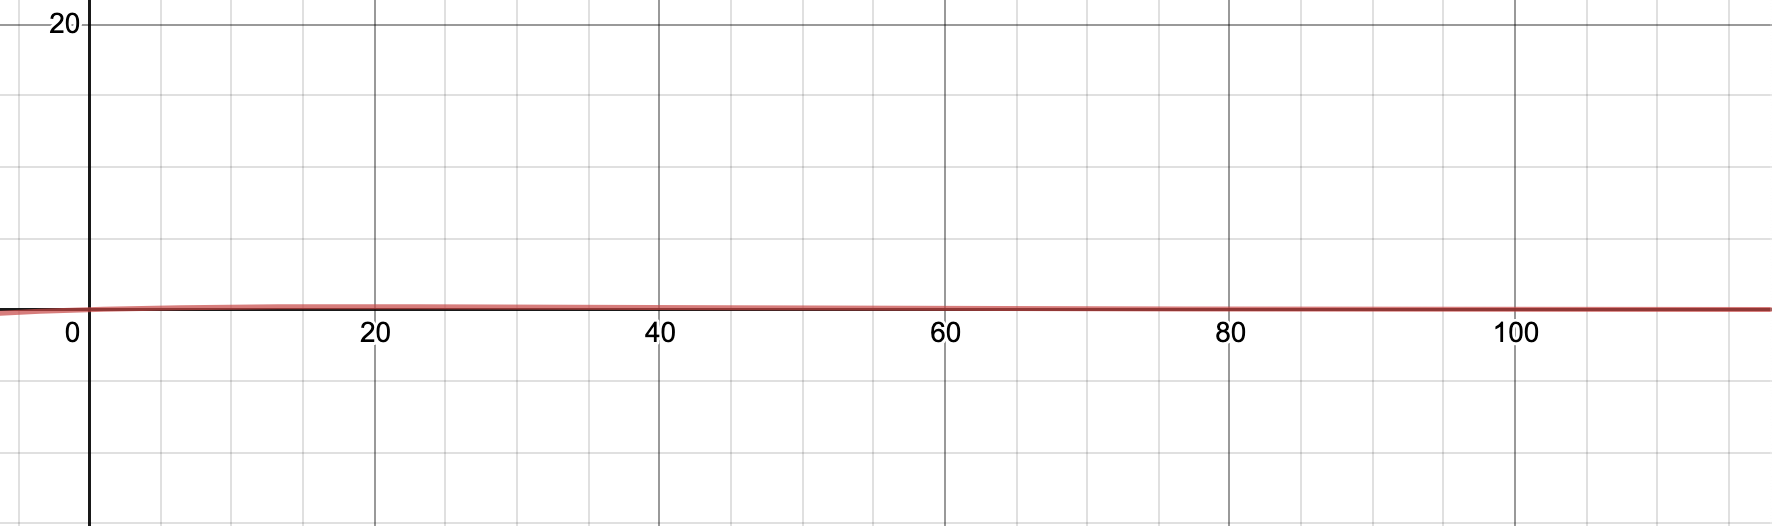
\includegraphics[scale = 0.6]{F(t)_3.png}}
		\end{center}
		\caption{График функции $F(t) = \frac{0.2}{19}t e^{-(\frac{t}{20} - 1)}$}
		\label{ris:F(t)_3}
	\end{figure}
	
	\newpage
	
	\subsection*{Задание 2.}
	
	\textit{График зависимости температуры $T(0, t)$ при 3-4 значениях параметров $a_2$ и/или $b_2$ теплоемкости.}
	
	\textit{Справка. С ростом теплоемкости темп нарастания температуры снижается.}
	
	\subsubsection*{Решение}
	
	Ниже приведены графики температуры $T(0, t)$ при 4 значениях параметров $a_2$ теплоемкости.
	
	\begin{figure}[h!]
		\begin{center}
			{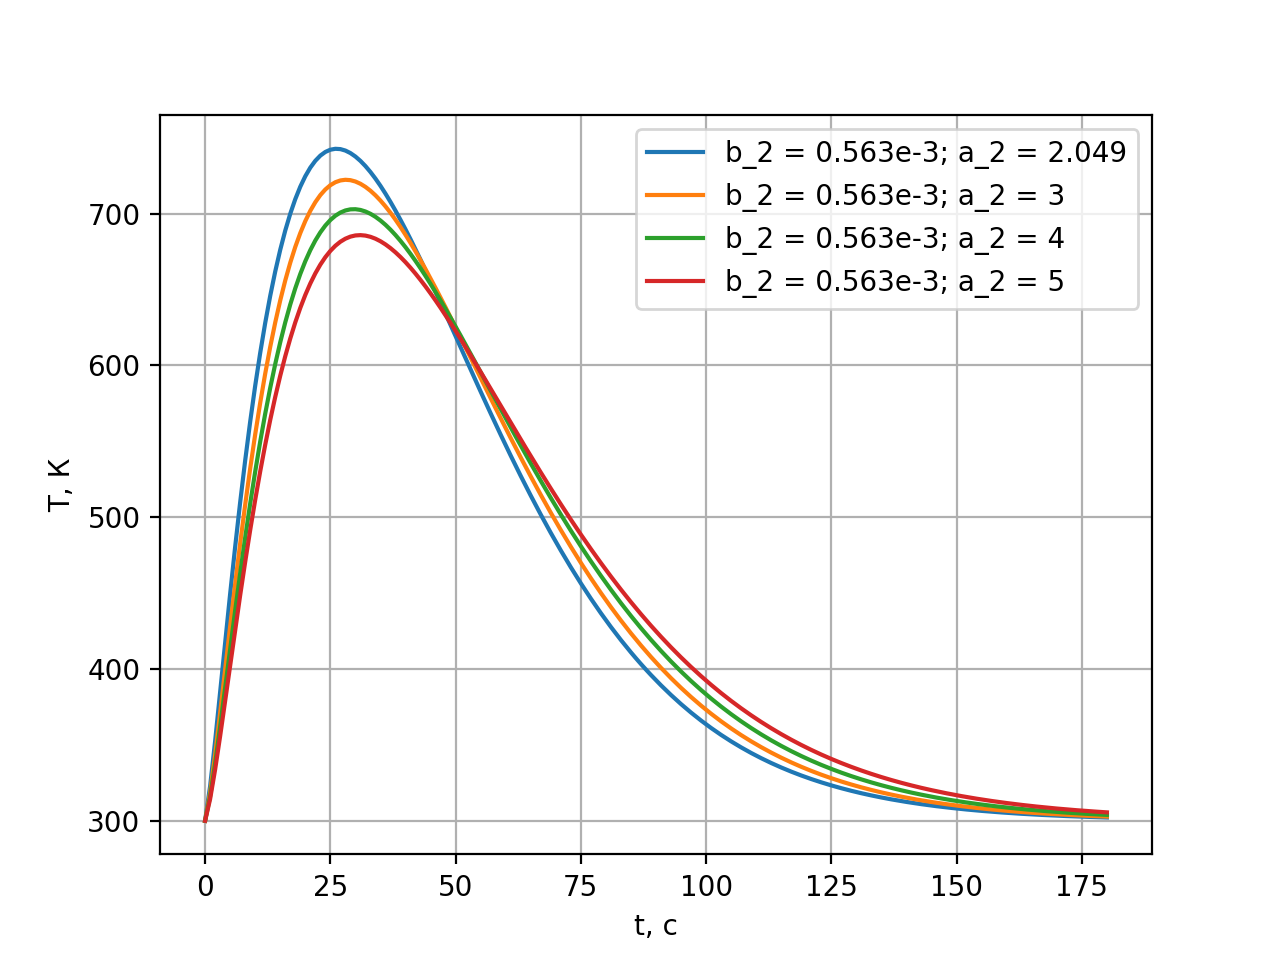
\includegraphics[scale = 0.8]{a_2_b_2.png}}
		\end{center}
		\caption{График функции $T(0, t)$ при $b_2 = 0.563e-3$}
		\label{ris:a_2_b_2}
	\end{figure}

	Как и указано в справке с ростом теплоемкости темп нарастания температуры снижается.
	
	\newpage
	
	\subsection*{Задание 3.}
	
	\textit{График зависимости температуры $T(0, t)$ (т.е. при $x = 0$ ) в частотном режиме теплового нагружения. Импульсы следуют один за другим с заданной частотой $\nu$ (частота определяется количеством импульсов в 1 секунду).}
	
	\textit{Показать, что при большом количестве импульсов температурное поле начинает в точности воспроизводиться от импульса к импульсу.}
	
	\textit{Продемонстрировать, как по мере роста частоты импульсов размах колебаний температуры уменьшается (вплоть до нуля), т.е. реализуется квазистационарный режим, при котором в торец поступает постоянный поток $F_c = \nu \int_{0}^{t_u}F(t)dt$. Здесь $t_u$ - длительность импульса, определяемая как момент времени, когда $\frac{F(t_u)}{F_{max}} \approx 0.05$. Если взять прямоугольные импульсы длительностью $t_u$, т.е. $F(t) = const = F_0$, то $F_c = \nu F_0 t_u$.}
	
	\textit{Справка. Полученное температурное поле должно совпасть с результатом расчета $T(x)$ по программе лаб. работы №3 при $F_0 = F_c$, разумеется при всех одинаковых параметрах модели, в частности, вместо $k(T)$ надо использовать $k(x)$ из лаб. работы №3.}
	
	\subsubsection*{Решение}
	
	Частотный режим реализуется следующим образом:
	\begin{itemize}
		\item Заводится массив $pulses_t$ для $t_i$, содержаший информацию о том, сколько прошло времени с момента запуска $i-ого$ импульса.
		\item В момент времени $T = \frac{1}{\nu}$, заносится в массив текущее значение времени $t$.
		
		Затем происходит обнуление t (запускается следующий импульс).
		\item $F(t)$ находится как сумма текущей волны и всех предыдущих, состояние которых лежит в массиве $pulses_t$.
		\item В конце каждой итерации по времени происходит увеличение всех элементов массива $pulses_t$ на $\tau$ (обновляется состояние каждого импульса).
	\end{itemize}

	\newpage

	Ниже приведен график зависимости $T(0, t)$ в частотном режиме теплого нагружения при $\nu = 0.01$ (т. е. второй импульс запускается, когда $t = 100$ с.); $F_{max}=50$ Вт/см$^2$;$t_{max} = 20$ с.:
	
	\begin{figure}[h!]
		\begin{center}
			{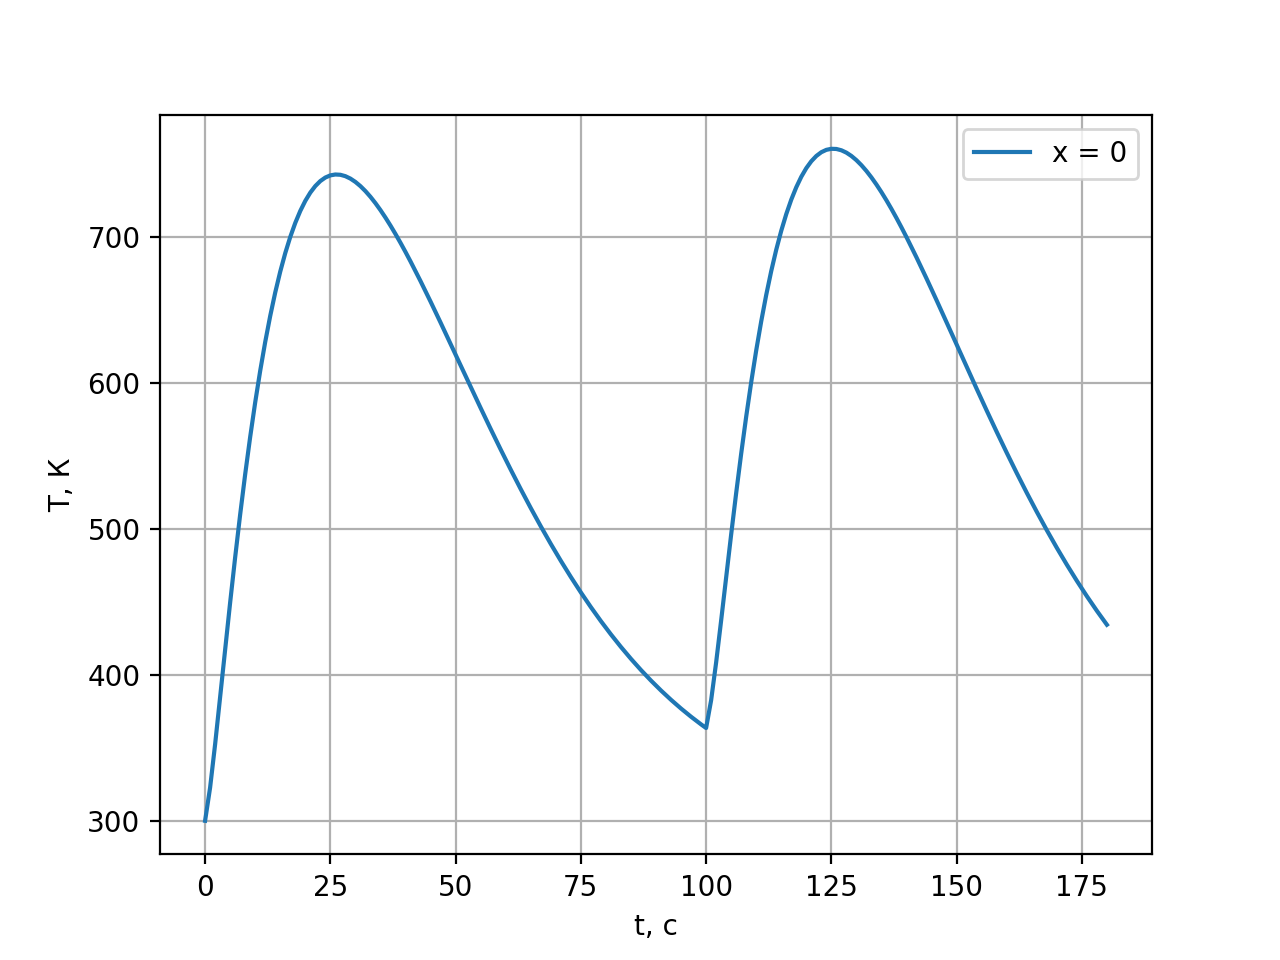
\includegraphics[scale = 0.7]{nu=0.01.png}}
		\end{center}
		\caption{График функции $T(0, t)$ при $\nu=0.01$. $F_{max}=50$ Вт/см$^2$; $t_{max} = 20$ с.}
		\label{ris:nu=0.01}
	\end{figure}

	Видно, что во время достижения амплитуды второго импульса, температура больше, чем во время достижения первого импульса. Это говорит о том, что к этому моменту времени первый импульс еще не успел до конца затухнуть.
	
	\newpage
	
	Ниже приведены графики зависимости $T(0, t)$ в частотном режиме теплого нагружения с постепенным увеличением частоты от $\nu = 0.05$ с. до $\nu = 0.5$ 1/с. с шагом 0.05 1/с.. $F_{max}=5$ Вт/см$^2$(уменьшено в 10 раз, поскольку в условиях задачи сказано, что решения, в которых температура превышает значения примерно 2000К, физического смысла не имеют и практического интереса не представляют.); $t_{max} = 20$ с.:
	
	\begin{figure}[h!]
		\begin{minipage}[b]{0.55\textwidth}
			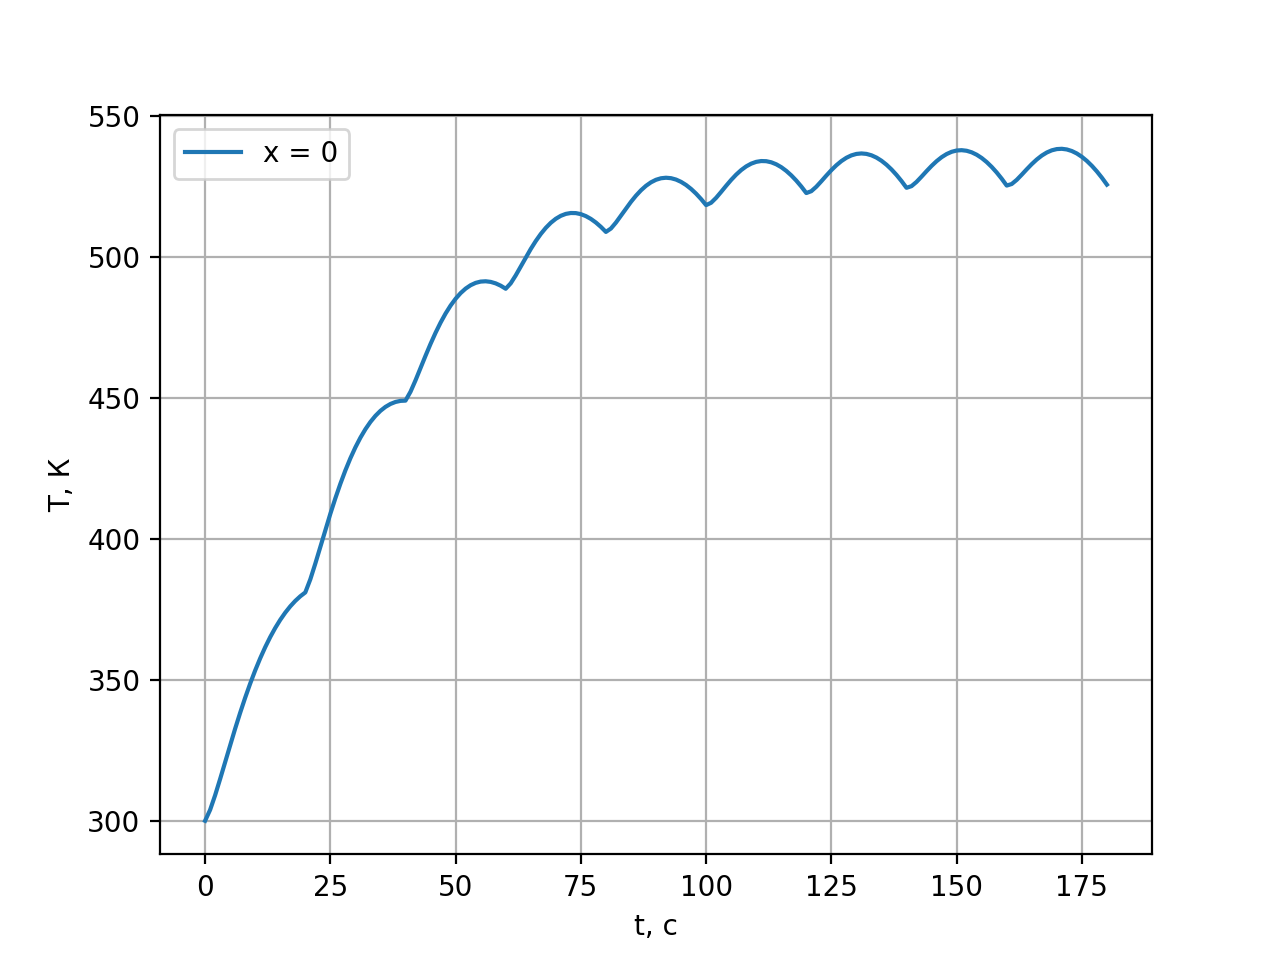
\includegraphics[width=\textwidth]{nu=0.05.png}
			\center{График функции $T(0, t)$ при $\nu=0.05$ 1/с. $F_{max}=5$ Вт/см$^2$; $t_{max} = 20$ с.}
		\end{minipage}
		\begin{minipage}[b]{0.55\textwidth}
			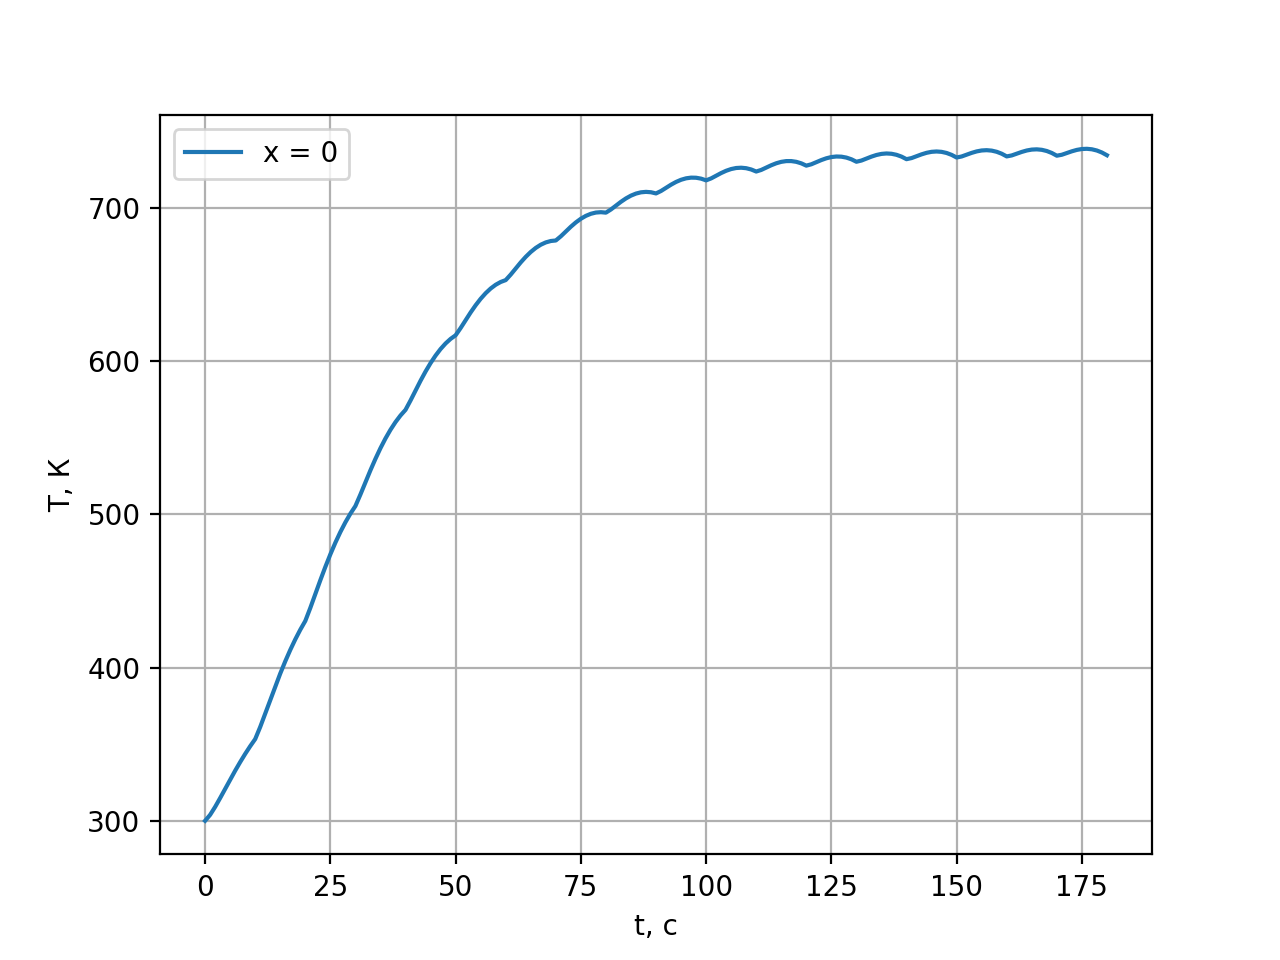
\includegraphics[width=\textwidth]{nu=0.1.png}
			\center{График функции $T(0, t)$ при $\nu=0.1$ 1/с. 
				
				$F_{max}=5$ Вт/см$^2$; $t_{max} = 20$ с.}
		\end{minipage}
		\label{ris:nu=0.05-0.1}
	\end{figure}


	\newpage

	\begin{figure}[h!]
		\begin{minipage}[b]{0.55\textwidth}
			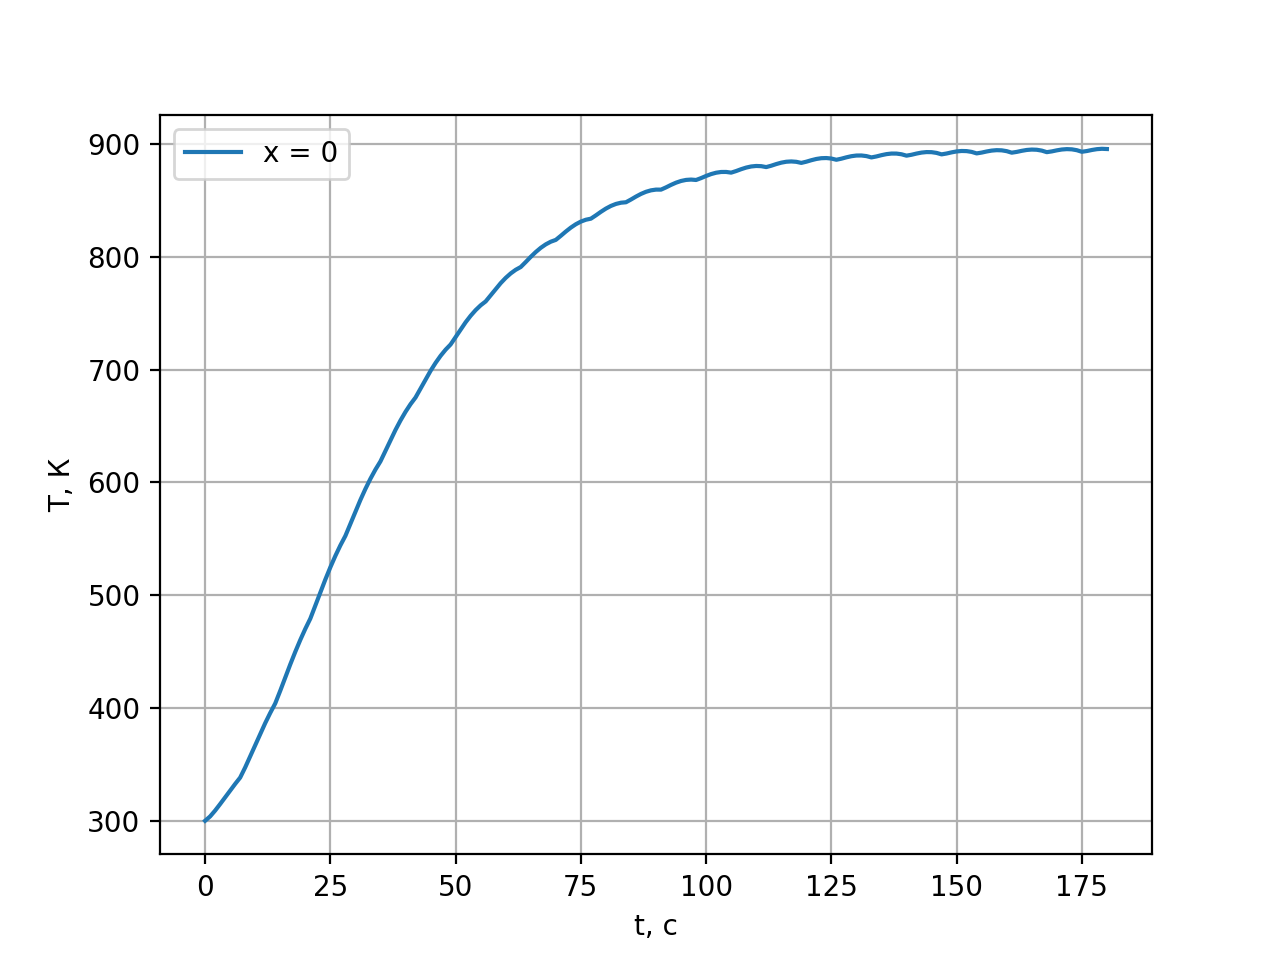
\includegraphics[width=\textwidth]{nu=0.15.png}
			\center{График функции $T(0, t)$ при $\nu=0.15$ 1/с. $F_{max}=5$ Вт/см$^2$; $t_{max} = 20$ с.}
		\end{minipage}
		\begin{minipage}[b]{0.55\textwidth}
			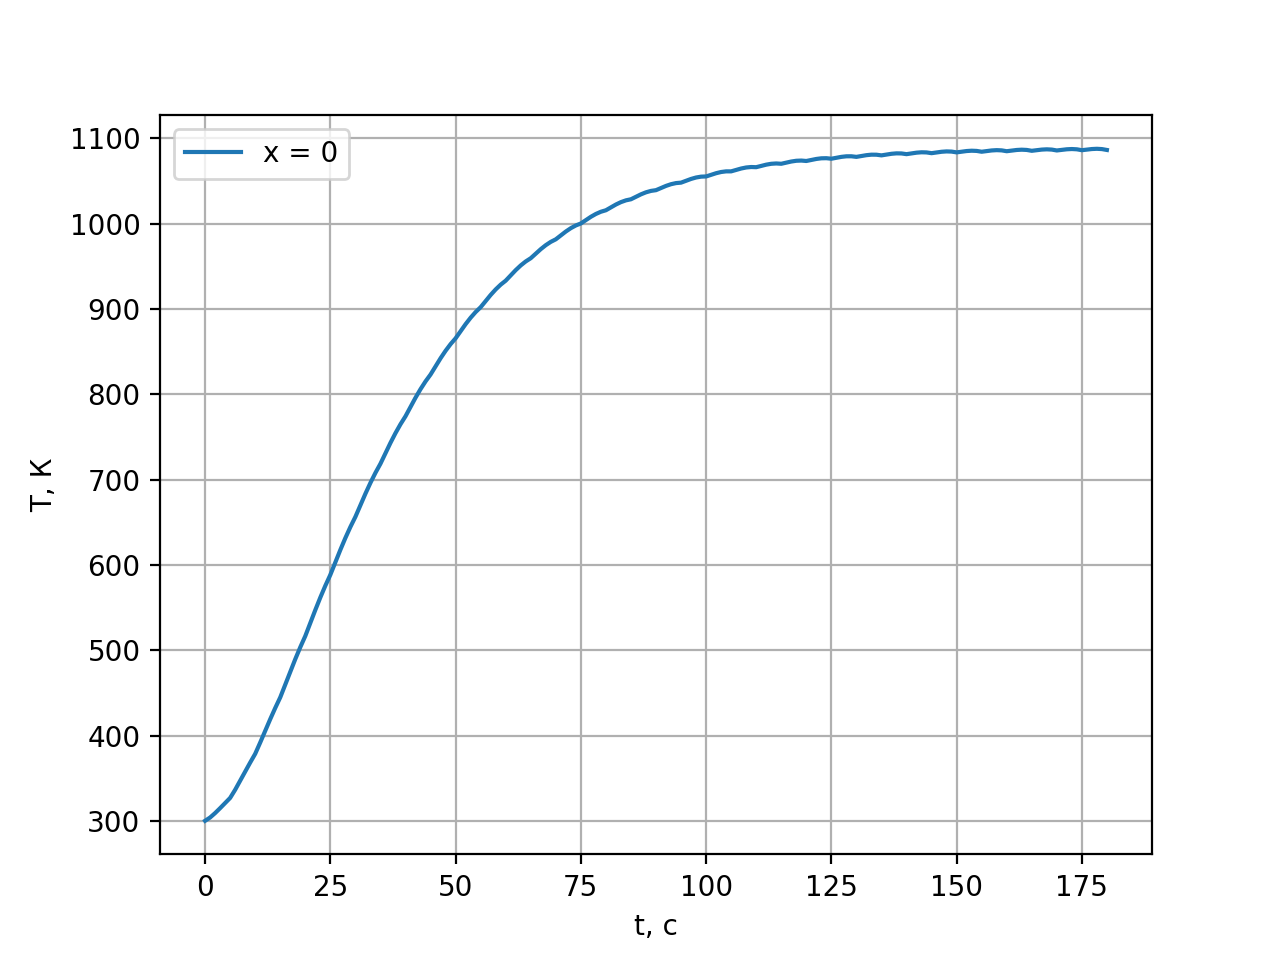
\includegraphics[width=\textwidth]{nu=0.2.png}
			\center{График функции $T(0, t)$ при $\nu=0.2$ 1/с. 
				
				$F_{max}=5$ Вт/см$^2$; $t_{max} = 20$ с.}
		\end{minipage}
		\label{ris:nu=0.15-0.2}
	\end{figure}

	\begin{figure}[h!]
		\begin{minipage}[b]{0.55\textwidth}
			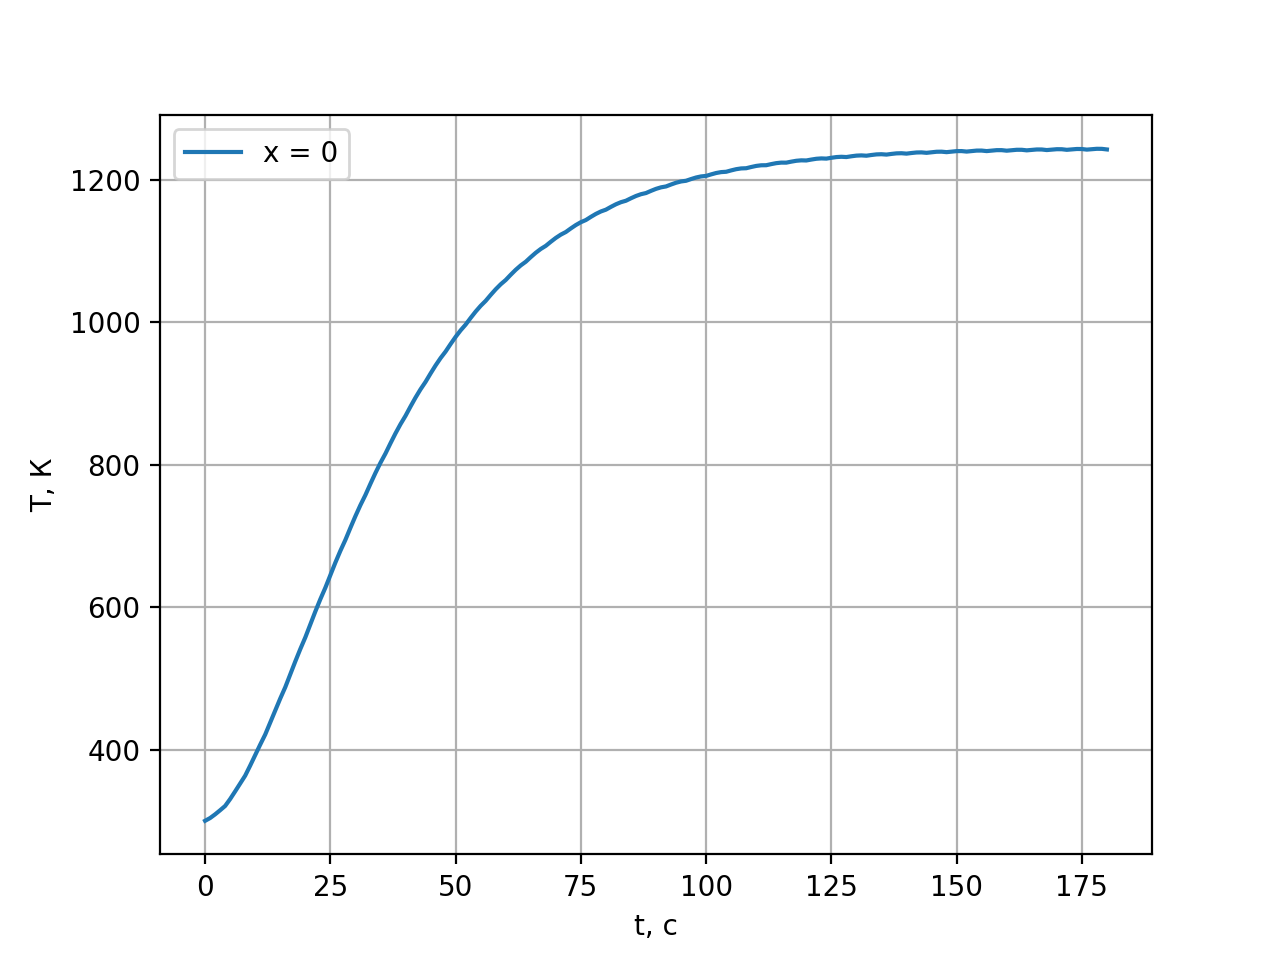
\includegraphics[width=\textwidth]{nu=0.25.png}
			\center{График функции $T(0, t)$ при $\nu=0.25$ 1/с. $F_{max}=5$ Вт/см$^2$; $t_{max} = 20$ с.}
		\end{minipage}
		\begin{minipage}[b]{0.55\textwidth}
			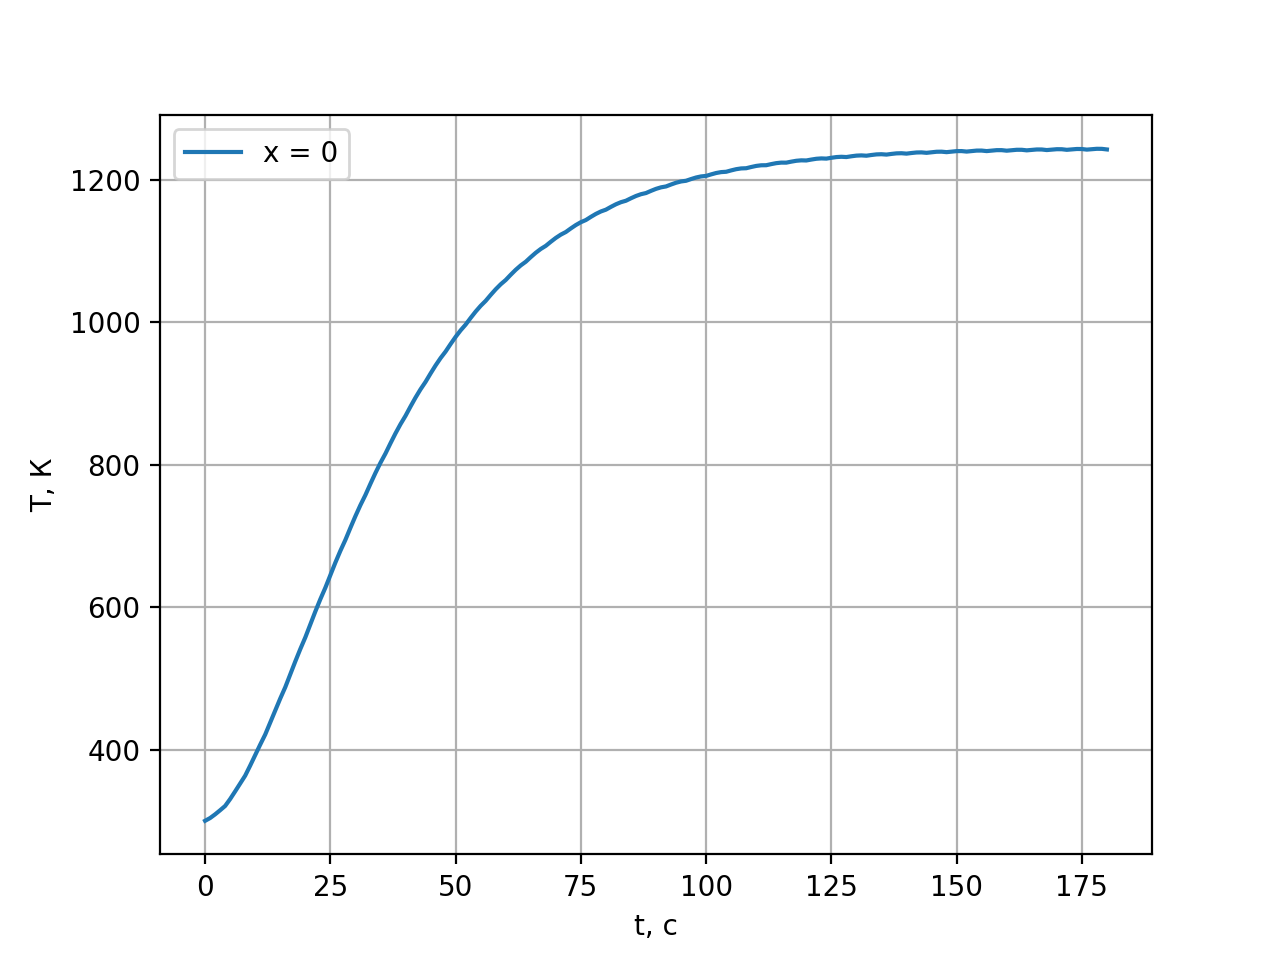
\includegraphics[width=\textwidth]{nu=0.3.png}
			\center{График функции $T(0, t)$ при $\nu=0.3$ 1/с. 
				
				$F_{max}=5$ Вт/см$^2$; $t_{max} = 20$ с.}
		\end{minipage}
		\label{ris:nu=0.25-0.3}
	\end{figure}

	\newpage

	\begin{figure}[h!]
		\begin{minipage}[b]{0.55\textwidth}
			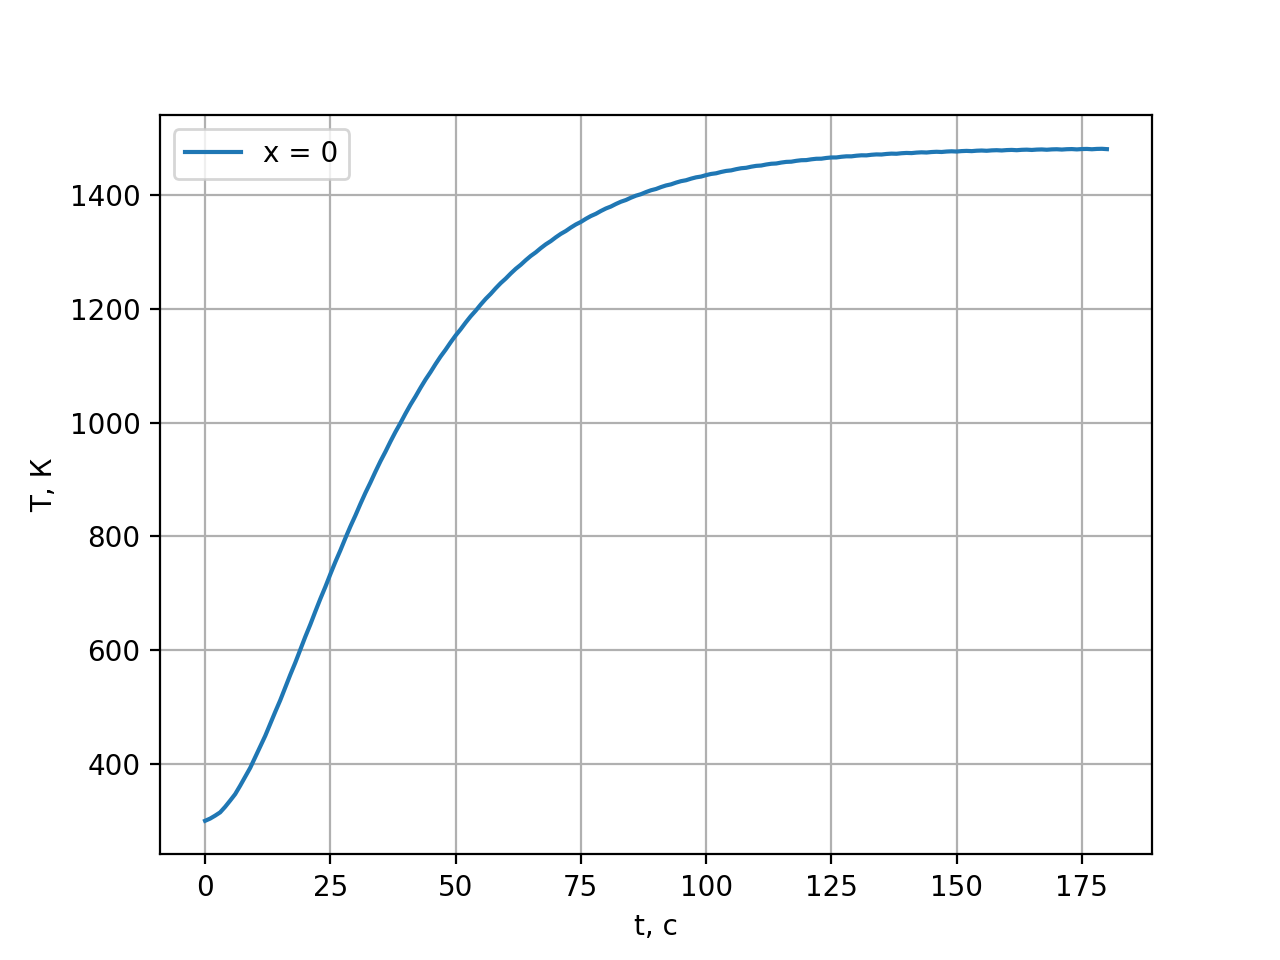
\includegraphics[width=\textwidth]{nu=0.35.png}
			\center{График функции $T(0, t)$ при $\nu=0.35$ 1/с. $F_{max}=5$ Вт/см$^2$; $t_{max} = 20$ с.}
		\end{minipage}
		\begin{minipage}[b]{0.55\textwidth}
			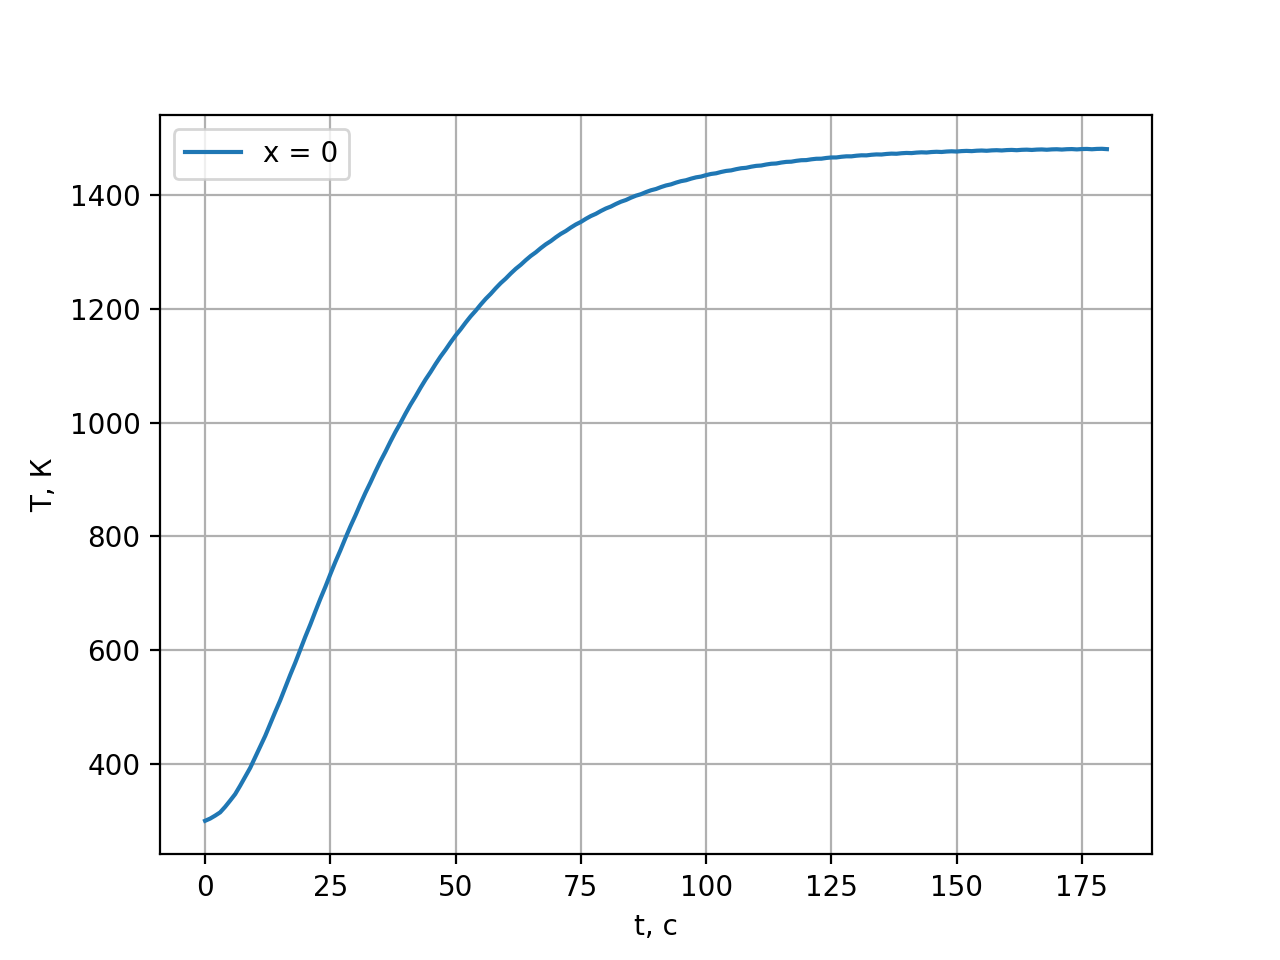
\includegraphics[width=\textwidth]{nu=0.4.png}
			\center{График функции $T(0, t)$ при $\nu=0.4$ 1/с. 
				
				$F_{max}=5$ Вт/см$^2$; $t_{max} = 20$ с.}
		\end{minipage}
		\label{ris:nu=0.35-0.4}
	\end{figure}

	\begin{figure}[h!]
		\begin{minipage}[b]{0.55\textwidth}
			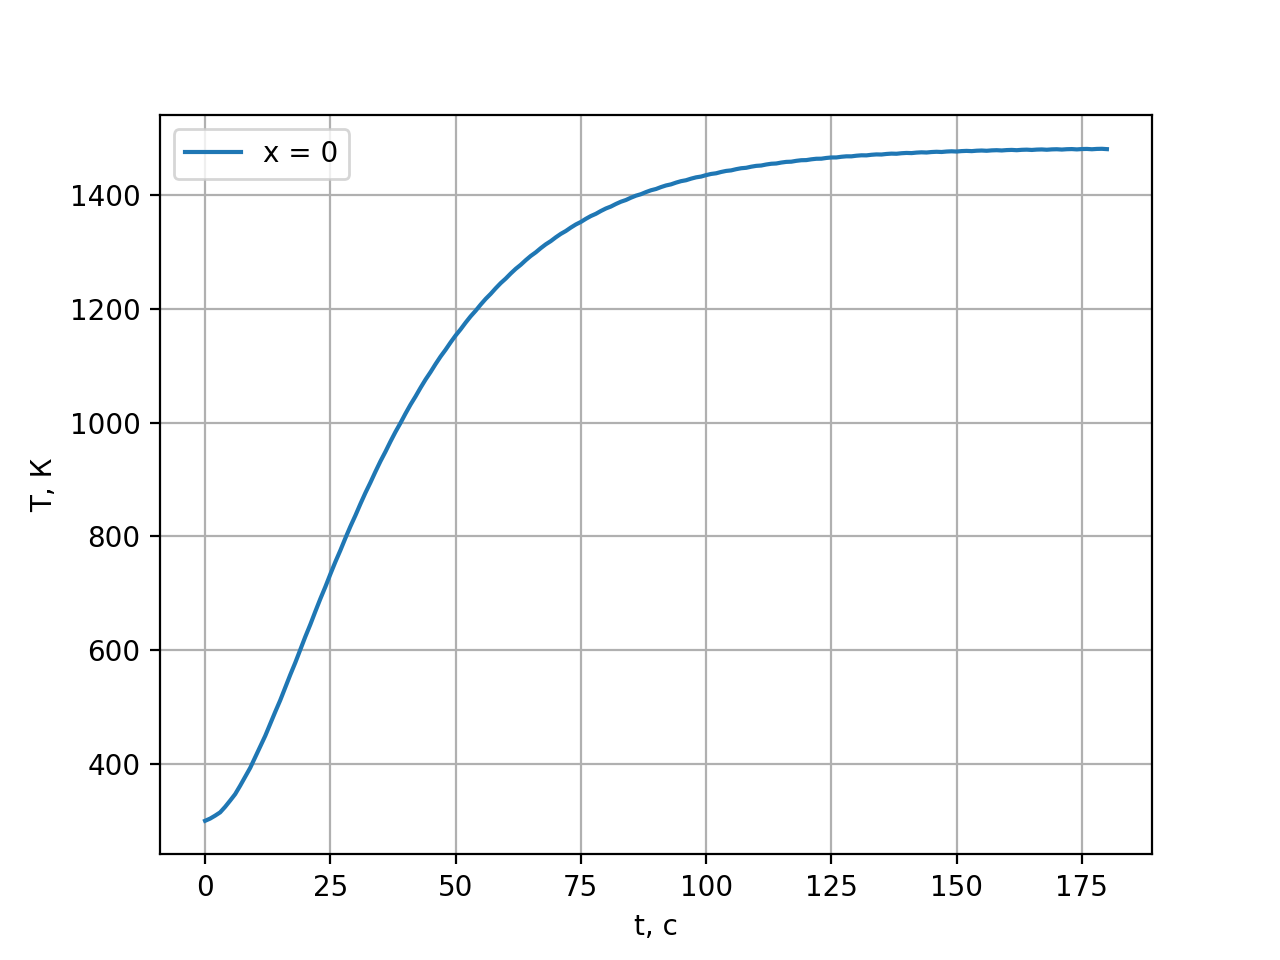
\includegraphics[width=\textwidth]{nu=0.45.png}
			\center{График функции $T(0, t)$ при $\nu=0.45$ 1/с. $F_{max}=5$ Вт/см$^2$; $t_{max} = 20$ с.}
		\end{minipage}
		\begin{minipage}[b]{0.55\textwidth}
			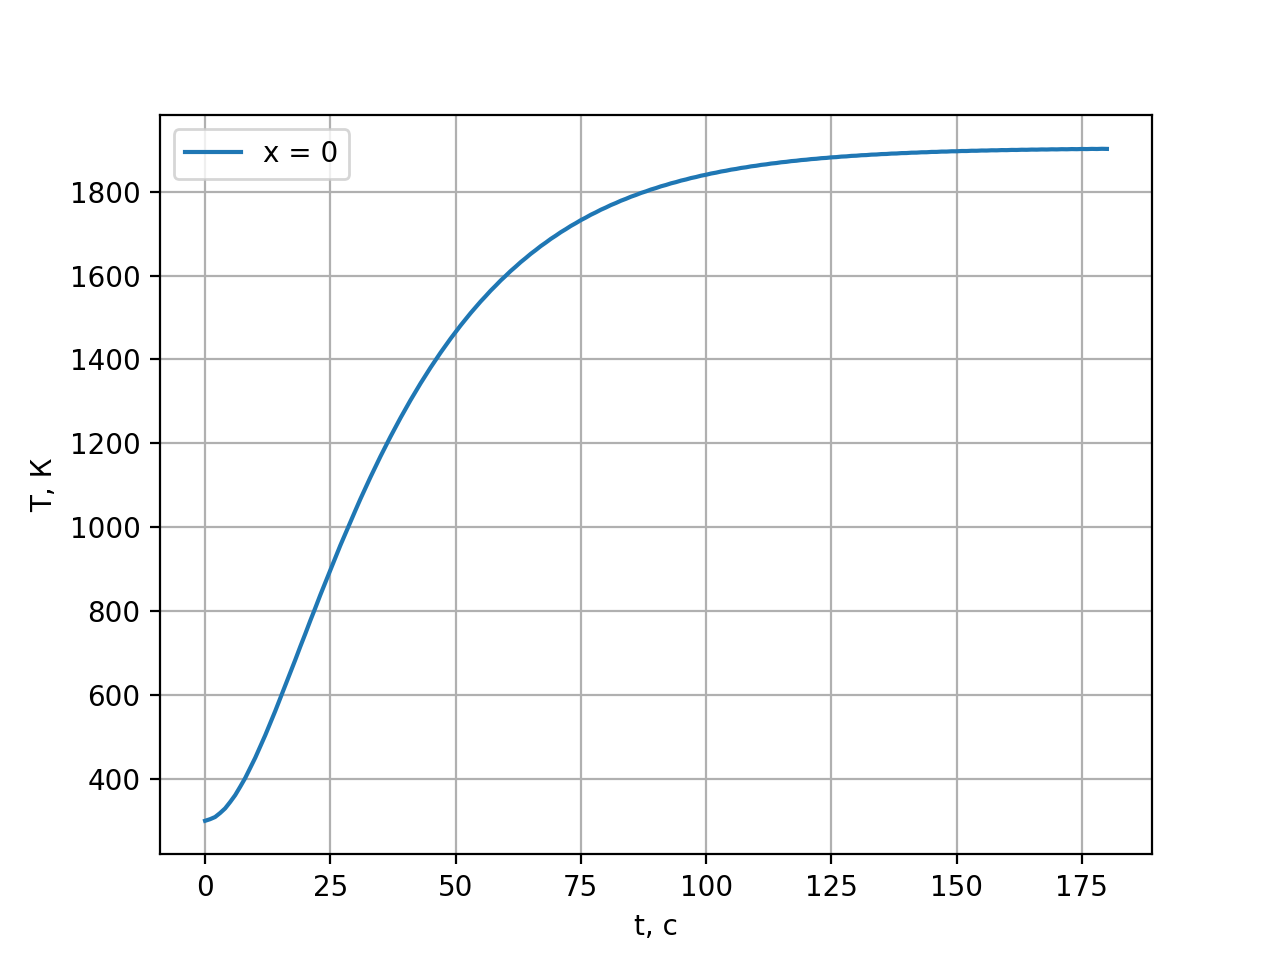
\includegraphics[width=\textwidth]{nu=0.5.png}
			\center{График функции $T(0, t)$ при $\nu=0.5$ 1/с. 
				
				$F_{max}=5$ Вт/см$^2$; $t_{max} = 20$ с.}
		\end{minipage}
		\label{ris:nu=0.45-0.5}
	\end{figure}
	
	Видно, что при $\nu = 0.5$ 1/с температурное поле в точности воспроизводиться от импульса к импульсу.
	
	
	Возьмем $k(x)$ из лаб. работы №3 вместо $k(T)$. Остальные параметры оставим такими же.
	При $t_u = 115.0$ с. $\frac{F(t_u)}{F_{max}} \approx 0.05$. 
	
	Следовательно, $F_c = 0.5 \int_{0}^{115.0} \frac{5}{20}t e^{- (\frac{t}{20} - 1)}dt = 132.994$ К. 

	\newpage

	Ниже приведен график распределения $T(0, t)$ при описанных выше параметрах.
	
	\begin{figure}[h!]
		\begin{center}
			{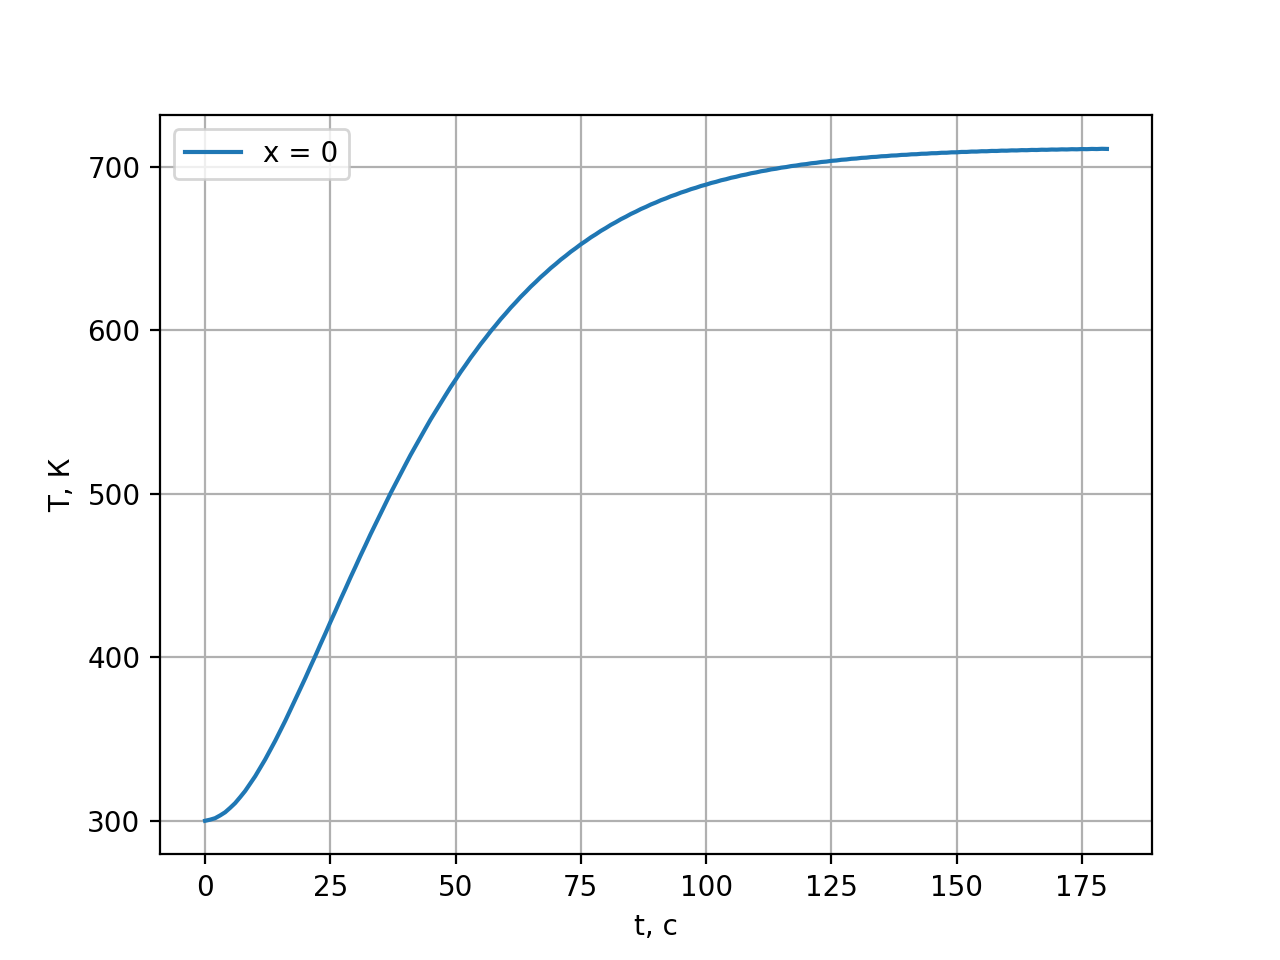
\includegraphics[scale = 0.7]{nu=0.5;k(x).png}}
		\end{center}
		\caption{График функции $T(0, t)$ при $\nu=0.5$. $F_{max}=5$ Вт/см$^2$; $t_{max} = 20; k(x)$ с.}
		\label{ris:nu=0.5;k(x)}
	\end{figure}
	
	Видно, что при установлении квазистационарного режима $T \approx 710$ К, что совпадает с результатом расчета $T(x)$ по программе лаб. работы №3 при $F_0 = F_c$.

	\textit{Примечание:}
	
	\textit{Все измерения в текущем задании были сделаны при оптимальных шагах $h = 0.01$ см.; $\tau = 1$ с., полученных в задании 1.}
	
\end{document}